\documentclass[12pt,a4paper]{article}

\usepackage[margin=2.5cm]{geometry}
\usepackage{amsmath,amssymb}
\usepackage{graphicx}
\usepackage{booktabs}
\usepackage{hyperref}
\usepackage{xcolor}
\usepackage{caption}
\usepackage{subcaption}
\usepackage{array}
\usepackage{float}
\usepackage{parskip}

\hypersetup{
  colorlinks=true,
  linkcolor=blue!70!black,
  citecolor=green!50!black,
  urlcolor=blue!70!black
}

\title{Search for $\Sigma^0$ Hyperon Production\\
       in Anti-Neutrino Interactions at MicroBooNE}
\author{J.~Nowak}
\date{June 2026}

\begin{document}

\maketitle
\tableofcontents
\clearpage

%% ============================================================
\section{Introduction}
%% ============================================================

Strange-particle production in neutrino--nucleus interactions provides
a sensitive test of the electroweak current structure and nuclear effects
at energies relevant to the oscillation experiments of the short- and
long-baseline programmes.  The neutral Sigma hyperon, $\Sigma^0$, is
the lightest strange baryon accessible via charged-current (CC)
anti-neutrino scattering off nucleons and has not yet been observed in
neutrino experiments.

The $\Sigma^0$ carries isospin $I = 1$, strangeness $S = -1$, and decays
electromagnetically with a branching fraction of essentially 100\%:
\begin{equation}
  \Sigma^0 \;\to\; \Lambda + \gamma
  \qquad (\tau \approx 7.4\times10^{-20}~\text{s})\,.
  \label{eq:sigma_decay}
\end{equation}
The subsequent weak decay $\Lambda \to p + \pi^-$ (branching fraction
$63.9\,\%$) yields a fully charged-particle final state alongside the
hard photon, making the reaction observable in a fine-grained detector.
The complete signal topology studied here is therefore
\begin{equation}
  \bar\nu_\mu + N \;\to\; \mu^+ + \Sigma^0 \;,\quad
  \Sigma^0 \to \Lambda + \gamma \;,\quad
  \Lambda \to p + \pi^-\,,
  \label{eq:signal}
\end{equation}
giving four visible final-state objects: a muon ($\mu^+$), a proton
($p$), a charged pion ($\pi^-$), and a photon ($\gamma$).

The associated production mechanism $\bar\nu_\mu\,p \to \mu^+\,\Sigma^0$
proceeds via the charged weak current with strangeness change
$|\Delta S| = 1$ and is Cabibbo suppressed relative to quasi-elastic
scattering by a factor $\tan^2\theta_C \approx 0.05$.  Theoretical
predictions for the total cross section span a range of
$\mathcal{O}(10^{-40})$~cm$^2$ at neutrino energies of $\sim 1$~GeV.
A positive observation, or a stringent upper limit, constrains
hyperon-production models that feed into flux-averaged oscillation
analyses.

Additionally, the $\Sigma^0$ search requires simultaneous reconstruction
of three tracks and one electromagnetic shower, exercising the full
particle-identification capabilities of a liquid-argon time projection
chamber (LArTPC) in a way that benefits reconstruction algorithm
development.

\subsection{Cross-Section Theory and Intranuclear Rescattering}
\label{sec:theory}

The elementary cross section for $\bar\nu_\mu\,p\to\mu^+\,\Sigma^0$ is
derived from the $V{-}A$ structure of the electroweak Standard Model.
The hadronic matrix element is parametrised by six Lorentz-invariant
form factors consistent with SU(3) flavour
symmetry~\cite{Thorpe:2020sbx,Alam:2014jza}:
\begin{itemize}
  \item Two isovector \emph{vector} form factors $f_1(Q^2)$ and $f_2(Q^2)$,
        determined from nucleon electromagnetic data via the
        Ademollo--Gatto theorem;
  \item One dominant \emph{axial} form factor
        $g_1(Q^2)=g_1^{(0)}(1+Q^2/M_A^2)^{-2}$ with axial mass
        $M_A\simeq1.026$~GeV, with $g_1^{(0)}$ fixed from semileptonic
        hyperon decay data assuming SU(3) symmetry;
  \item A \emph{pseudoscalar} form factor $g_3$ linked to $g_1$ via PCAC;
  \item \emph{Second-class current} (SCC) form factors $f_3$ and $g_2$,
        forbidden by $G$-parity in the SU(2) limit but receiving
        non-zero contributions from SU(3) symmetry breaking.
\end{itemize}
The amplitude is suppressed relative to the $\bar\nu_\mu\,n\to\mu^+\,n$
quasielastic channel by the CKM factor
$|V_{us}|^2/|V_{ud}|^2\approx\tan^2\theta_C\approx 0.053$
($|V_{us}|\simeq0.2248$), which explains the small predicted cross sections.

A detailed study of these effects for argon and carbon targets was
performed by Thorpe, Nowak \emph{et al.}~\cite{Thorpe:2020sbx} using
the NuWro generator.  Key findings include: a $\pm10\,\%$ variation in
$M_A$ shifts the total cross section by $\pm15$--$20\,\%$; SCC
contributions are below $5\,\%$ but alter the muon angular distribution
at low neutrino energies; and SU(3)-breaking effects at the $20\,\%$
level provide the dominant theory uncertainty.

\textbf{Intranuclear rescattering.}
The $\Sigma^0$ decays electromagnetically with a lifetime
$\tau(\Sigma^0)\approx7.4\times10^{-20}$~s, corresponding to a
rest-frame mean decay length $c\tau_0\approx22\,\mu$m.  This is many
orders of magnitude larger than the Ar nuclear diameter
($\sim8$~fm $\simeq8\times10^{-13}$~cm), yet it represents a
probability of only $\sim2\times10^{-4}$ that the $\Sigma^0$ decays
inside the primary nucleus before escaping.  In practice, the $\Sigma^0$
escapes and decays to $\Lambda+\gamma$ in the liquid argon at a
microscopically displaced position unresolvable by the LArTPC.

The $\Lambda$ produced from $\Sigma^0\to\Lambda\gamma$ propagates with
$c\tau(\Lambda)\approx7.9$~cm, forming a macroscopic secondary vertex
($p+\pi^-$) observable in the detector.  While traversing the liquid
argon, the $\Lambda$ may undergo hadronic interactions (nuclear
interaction length $\lambda_\text{int}^\text{LAr}\approx84$~cm); the
probability of interaction before the weak decay is approximately
$10$--$15\,\%$, reducing the signal efficiency.  This attenuation is
fully accounted for in the \textsc{Geant4} simulation.

A distinct FSI mechanism that creates background is
$\Sigma\to\Lambda$ charge-exchange conversion of
\emph{co-produced} $\Sigma^{\pm}$ hyperons:
$\Sigma\,N\to\Lambda\,N$ inside the primary nucleus.
Since the $\Sigma^+$ and $\Sigma^-$ have hadronic lifetimes
($c\tau\approx2$--$4$~cm), they can rescatter before escaping
the nucleus and convert to $\Lambda$, producing events where the
topology mimics the $\Sigma^0$ signal.  As quantified in
Ref.~\cite{Thorpe:2020sbx}, such conversions significantly
enhance the apparent $\Lambda$ yield and constitute the dominant
contribution to the ``Hyperons'' background category
(4.9\,\% at the final selection stage, see Section~\ref{sec:xsec}).

\subsection{Prior Experimental and Theoretical Results}
\label{sec:prior}

No experimental observation of $\Sigma^0$ production in neutrino
interactions has previously been reported.  The Cabibbo-suppressed
$\Lambda$ production channel
$\bar\nu_\mu\,N\to\mu^+\,\Lambda(+X)$ is the phenomenologically
closest process.

\textbf{Theoretical predictions.}
Mintz and Wen~\cite{Mintz:2006un} provided early predictions for the
total and differential cross sections of
$\bar\nu_\mu\,p\to\mu^+\,\Lambda$ and
$\bar\nu_\mu\,p\to\mu^+\,\Sigma^0$ on free nucleons using SU(3) form
factors.  Alam \emph{et al.}~\cite{Alam:2014jza} extended the
calculation to nuclei ($^{12}$C, $^{40}$Ar, $^{56}$Fe, $^{208}$Pb)
within a local-density approximation including Fermi motion, Pauli
blocking, and hyperon--nucleon FSI.  Thorpe, Nowak \emph{et al.}~\cite{Thorpe:2020sbx}
provided flux-averaged NuWro predictions for BNB and DUNE on argon,
studying the sensitivity to $M_A$, SCC, and SU(3) violations.
Benitez~Galan \emph{et al.}~\cite{BenitezGalan:2023hyi} recently
found that the $\Sigma^*(1385)$ resonance contributes approximately
one-third of the inclusive $\Lambda$ production cross section at
MicroBooNE energies, highlighting the importance of resonant channels.

\textbf{First $\Lambda$ measurement at MicroBooNE.}
Using the same $4.9\times10^{20}$~PoT NuMI RHC data set
as this analysis, the MicroBooNE collaboration reported the first
measurement of CC quasielastic $\Lambda$
production~\cite{MicroBooNE:2022ctm}.  Five candidate events were
observed against a GENIE prediction of $5.3\pm1.1$, yielding a
flux-averaged cross section
\begin{equation}
  \sigma(\bar\nu_\mu\,\text{Ar}\to\mu^+\,\Lambda)\cdot
  \text{Br}(\Lambda\to p\pi^-)
  \;=\; 2.0^{+2.2}_{-1.7}\times10^{-40}~\text{cm}^2/\text{Ar}
  \qquad (68\,\%~\text{CL})\,,
  \label{eq:lambda_meas}
\end{equation}
consistent with GENIE at the $1\sigma$ level and constituting the
world's first measurement of this Cabibbo-suppressed channel.
This result validates the hyperon reconstruction tools employed in
the present $\Sigma^0$ search.

%% ============================================================
\section{The MicroBooNE Experiment}
%% ============================================================

\subsection{Detector}

MicroBooNE~\cite{Acciarri:2016smi} is a single-phase LArTPC located at
Fermi National Accelerator Laboratory (Fermilab) at a baseline of 470~m
from the Booster Neutrino Beam (BNB) target and 803~m from the NuMI
target at $7.3^\circ$ off-axis.  The active volume
contains $\approx 85$~tonnes of liquid argon with dimensions
$2.56~\text{m}\;(\text{drift}) \times 2.33~\text{m}\;(\text{height})
\times 10.37~\text{m}\;(\text{length})$.

Ionisation electrons drift under a uniform electric field of
$\approx 273$~V/cm towards a readout anode consisting of three wire
planes (U, V induction; Y collection) with 3~mm wire spacing and
a total of 8256~wires.  Scintillation light is collected by 32
photomultiplier tubes (PMTs).  The combination of full 3D imaging,
continuous calorimetric readout, and $\mathcal{O}(\text{mm})$ spatial
resolution makes LArTPCs ideal for multi-particle final states.

\subsection{Fiducial Volume}

Events are required to have their reconstructed primary vertex within
a fiducial volume (FV) that excludes the first and last few centimetres
near each face:
\begin{align}
  3.00~\text{cm} &< x < 253.35~\text{cm}\,,\\
  -112.53~\text{cm} &< y < 114.47~\text{cm}\,,\\
  3.1~\text{cm} &< z < 1033.0~\text{cm}\,.
\end{align}
A dead region $z \in [675.1, 775.1]$~cm arising from a faulty wire
segment is excluded for signal MC at truth level.

\subsection{Beam and Data Sample}

This analysis uses Run~3b data corresponding to
$4.90 \times 10^{20}$~protons on target (PoT) from the NuMI beam
operating in Reverse Horn Current (RHC) mode.  The peak anti-neutrino
energy is $\approx 0.25$~GeV.

%% ============================================================
\section{Simulation}
%% ============================================================

\subsection{Monte Carlo Samples}

Four simulated samples are used, all scaled to the data PoT of
$4.90 \times 10^{20}$:

\begin{table}[H]
  \centering
  \caption{Monte Carlo samples used in the analysis. Scaling factors
           $w_s = \text{PoT}_{\text{data}}/\text{PoT}_{\text{MC}}$ are
           applied to normalise each sample to the data luminosity.}
  \label{tab:samples}
  \begin{tabular}{llrr}
    \toprule
    Label & Content & PoT [$10^{20}$] & Scale factor \\
    \midrule
    \textbf{Sigma MC}      & Signal + other hyperons & 552.0 & 0.00888 \\
    \textbf{Background MC} & Neutrino overlay         &   9.28 & 0.528   \\
    \textbf{Dirt MC}       & Out-of-FV interactions   &  17.30 & 0.283   \\
    \textbf{Data}          & NuMI RHC anti-$\nu_\mu$  &   4.90 & 1.000   \\
    \bottomrule
  \end{tabular}
\end{table}

The signal and hyperon samples are generated using a dedicated
hyperon-production generator in the NuMI RHC flux, with GENIE~\cite{Andreopoulos:2009rq}
handling neutrino cross sections.  The background overlay sample
uses NuMI neutrino interactions embedded in real beam-off data to
reproduce detector noise and pile-up accurately.  The dirt sample
covers interactions in the surrounding material outside the cryostat.
Geant4~\cite{Agostinelli:2002hh} propagates all final-state particles
through the detector geometry, and LArSoft~\cite{Snider:2017wjd}
handles digitisation and reconstruction.

\subsection{Signal Definition}

A simulated event is classified as signal if it satisfies all of:
\begin{itemize}
  \item the incoming neutrino is an anti-muon-neutrino ($\bar\nu_\mu$, PDG $= -14$);
  \item a $\Sigma^0$ (PDG $= 3212$) is produced;
  \item the decay products include exactly one proton ($p_T > 0.3$~GeV/$c$)
        and one $\pi^-$ ($p_T > 0.1$~GeV/$c$);
  \item the true neutrino vertex lies within the fiducial volume and
        outside the dead region.
\end{itemize}
Events from the same MC file that do not satisfy these conditions form
the ``Hyperons'' background sub-sample (other hyperon species or
$\Sigma^0$ with $\Lambda \to n + \pi^0$).

%% ============================================================
\section{Event Reconstruction and Selection}
\label{sec:selection}
%% ============================================================

\subsection{Reconstruction Framework}

Particle reconstruction is performed with Pandora~\cite{Marshall:2015rfa},
a multi-algorithm pattern-recognition framework that clusters wire
hits into three-dimensional particle-flow objects (PFPs).  Each PFP
is assigned a track--shower score (0 = shower-like, 1 = track-like)
by a dedicated convolutional neural network.  Track-like PFPs are
fitted with a Kalman-filter track algorithm; shower-like PFPs are
reconstructed as electromagnetic showers.

Particle identification uses the log-likelihood ratio PID score
(\texttt{trk\_llrpid}), which combines $dE/dx$ measurements from
all three wire planes under signal and background hypotheses.  A
dedicated photon BDT score (\texttt{pfp\_photon\_bdt\_score})
separates cosmic and beam-induced photon showers from track stubs.

\subsection{Analysis Flow}

The selection proceeds in three stages:
\begin{enumerate}
  \item \textbf{Pre-selection cuts}: topology-based requirements that
        define the four-candidate event hypothesis ($\mu^+$, $\pi^-$,
        $p$, $\gamma$).
  \item \textbf{Quality and distance cuts}: threshold requirements on
        individual candidate properties and inter-candidate distances.
  \item \textbf{Multivariate classifier}: a Boosted Decision Tree (BDT)
        trained on 33~discriminating variables provides the final
        signal/background separation.
\end{enumerate}

\subsection{Candidate Selection Algorithm}

Candidates are chosen from the set of reconstructed PFPs:

\textbf{Muon candidate.}  The longest track-like PFP ($\text{score} > 0.8$)
within 20~cm of the primary vertex, with $\text{LLR PID} > 0.7$ and
length $> 10$~cm.

\textbf{Pion candidate.}  Among remaining track-like PFPs
($\text{score} > 0.5$), the one with the highest LLR PID score.
The pion is expected to have a positive (muon-like) LLR PID,
distinguishing it from the heavily ionising proton.

\textbf{Proton candidate.}  Among remaining track-like PFPs, the one
with the \emph{lowest} LLR PID score, consistent with heavy ionisation.

\textbf{Shower candidates.}  The two shower-like PFPs ($\text{score} < 0.5$)
closest to the primary vertex (excluding already-assigned candidates).
Shower~1 is the nearest, shower~2 the second nearest.

%% ============================================================
\section{Cut-Flow Selection}
%% ============================================================

\subsection{Sequential Cuts}

Table~\ref{tab:cutflow} summarises the cumulative effect of each selection
requirement.  All yields are scaled to $4.90 \times 10^{20}$~PoT.
Efficiency and purity are computed relative to all simulated events and
to the total background respectively.

\begin{table}[H]
  \centering
  \caption{Cut-flow table.  ``Bkg'' includes Background MC and Dirt MC.
           Purity $= S/(S+\text{Hyp}+\text{Bkg}+\text{Dirt})$.
           Efficiency $= S/S_0$ where $S_0 = 17.87$ is the total scaled
           signal.}
  \label{tab:cutflow}
  \setlength{\tabcolsep}{6pt}
  \begin{tabular}{lrrrrrr}
    \toprule
    Cut stage & $S$ & Hyp & Bkg & Dirt
              & Eff.\,[\%] & Purity\,[\%] \\
    \midrule
    All events       & 17.87 & 840.0 & 344\,824 & 99\,258 & 100.0 & 0.004 \\
    Fiducial vertex  & 14.63 & 696.4 & 145\,995 & 25\,992 &  81.9 & 0.008 \\
    $1 \le N_\gamma < 4$ & 10.48 & 415.7 &  53\,756 &  4\,549 &  58.7 & 0.018 \\
    Muon candidate   &  8.89 & 328.3 &  34\,250 &  2\,906 &  49.7 & 0.024 \\
    Pion candidate   &  6.98 & 270.1 &  25\,039 &    946 &  39.0 & 0.027 \\
    Proton candidate &  4.18 & 181.4 &  13\,654 &    240 &  23.4 & 0.030 \\
    $N_\text{tracks} < 5$ & 3.94 & 129.2 & 10\,966 & 224 & 22.1 & 0.035 \\
    Shower~1 quality &  3.63 &  76.3 &   7\,360 &    192 &  20.3 & 0.048 \\
    Distance cuts    &  3.07 &  48.5 &   4\,449 &     61 &  17.2 & 0.067 \\
    \midrule
    \textbf{BDTg $> 0.96$} & \textbf{1.04} & \textbf{0.05} & \textbf{0} & \textbf{0} & \textbf{5.8} & \textbf{95.1} \\
    \bottomrule
  \end{tabular}
\end{table}

\subsection{Individual Cut Definitions}

\textbf{C1 — Fiducial vertex.}
The reconstructed primary vertex must lie within the FV defined in
Section~2.2.

\textbf{C2 — Shower multiplicity.}
$1 \le N_\gamma \le 3$, requiring at least one shower (from the $\gamma$)
and rejecting events with $\ge 4$ showers which are dominated by $\pi^0$
backgrounds.

\textbf{C3 — Muon candidate.}
A track-like PFP satisfying $\text{score} > 0.8$, $\text{LLR PID} > 0.7$,
length $> 10$~cm, and vertex distance $< 20$~cm must exist.

\textbf{C4 — Pion candidate.}
At least one additional track-like PFP ($\text{score} > 0.5$) exists.

\textbf{C5 — Proton candidate.}
At least two additional track-like PFPs exist (one will be assigned as
proton).

\textbf{C6 — Track multiplicity.}
$N_\text{tracks} < 5$ to suppress multi-pion backgrounds.

\textbf{C7 — Shower~1 quality.}
$10 < N_{\text{hits},Y}^{\gamma_1} < 300$: the leading shower must be
genuine (not a stub) and not excessively large (rejecting $\pi^0$ showers).

\textbf{C8 — Distance cuts.}
The following pairwise distances must be satisfied simultaneously:
\begin{align*}
  d(\mu,\pi) &< 30~\text{cm}\,,\\
  d(p,\mu) &< 20~\text{cm}\,,\quad d(p,\pi) < 20~\text{cm}\,,\\
  d(\gamma_1,\mu) &< 100~\text{cm}\,,\quad
  d(\gamma_1,\pi) < 100~\text{cm}\,,\quad
  d(\gamma_1,p) < 100~\text{cm}\,.
\end{align*}
These requirements enforce that all candidates originate from a common
interaction vertex.

\subsection{Key Distributions After Pre-Selection}

Figure~\ref{fig:pid} shows the LLR PID scores for the three track
candidates after all pre-selection and distance cuts.  The muon candidate
correctly peaks near $+1$ for signal; the pion spans a broader range
reflecting the mixed ionisation of short pion tracks; the proton
candidate peaks near $-1$, consistent with heavy ionisation.

\begin{figure}[H]
  \centering
  \begin{subfigure}[b]{0.32\textwidth}
    \includegraphics[width=\textwidth]{figs/MuonPID.png}
    \caption{Muon LLR PID}
  \end{subfigure}
  \begin{subfigure}[b]{0.32\textwidth}
    \includegraphics[width=\textwidth]{figs/PionPID.png}
    \caption{Pion LLR PID}
  \end{subfigure}
  \begin{subfigure}[b]{0.32\textwidth}
    \includegraphics[width=\textwidth]{figs/ProtonPID.png}
    \caption{Proton LLR PID}
  \end{subfigure}
  \caption{LLR PID score distributions for the three track candidates
           after all pre-selection and distance cuts (Distances stage).
           Signal (red) is scaled up by the factor shown in the legend.
           Stacked histograms show other hyperons (green), background
           (blue), and dirt (grey).  All yields are normalised to
           $4.90\times10^{20}$~PoT.}
  \label{fig:pid}
\end{figure}

Figure~\ref{fig:kin} shows the shower multiplicity (after the fiducial
cut), the muon track length, and the first shower's distance from the
vertex after all distance cuts.

\begin{figure}[H]
  \centering
  \begin{subfigure}[b]{0.32\textwidth}
    \includegraphics[width=\textwidth]{figs/NShowers.png}
    \caption{Shower multiplicity}
  \end{subfigure}
  \begin{subfigure}[b]{0.32\textwidth}
    \includegraphics[width=\textwidth]{figs/MuonTrkLength.png}
    \caption{Muon track length [cm]}
  \end{subfigure}
  \begin{subfigure}[b]{0.32\textwidth}
    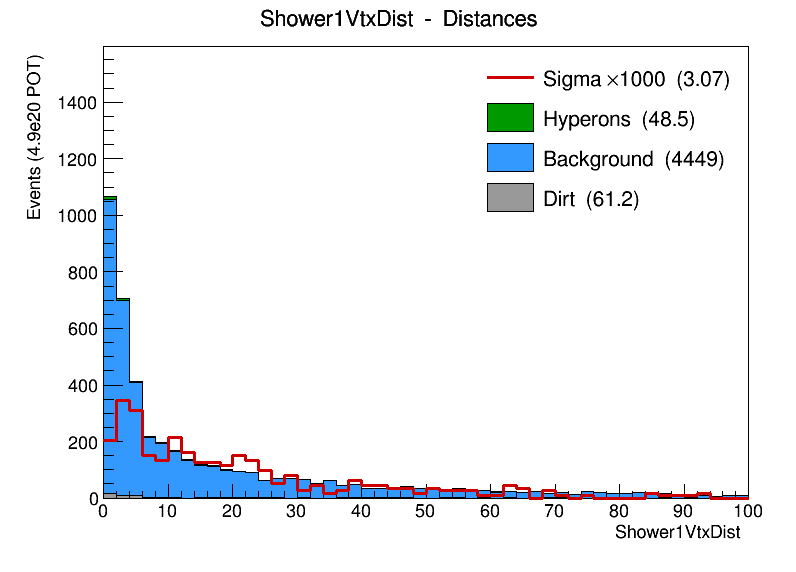
\includegraphics[width=\textwidth]{figs/Shower1VtxDist.png}
    \caption{Shower~1 distance from vertex [cm]}
  \end{subfigure}
  \caption{Selected kinematic distributions.  Left: number of reconstructed
           showers after the fiducial-vertex cut.  Centre and right: muon
           track length and leading-shower vertex distance after all
           pre-selection and distance cuts.}
  \label{fig:kin}
\end{figure}

Figure~\ref{fig:dedx} shows the $dE/dx$ in the collection plane (Y)
for the pion and proton candidates, two of the most discriminating
variables added in the MVA retraining.

\begin{figure}[H]
  \centering
  \begin{subfigure}[b]{0.45\textwidth}
    \includegraphics[width=\textwidth]{figs/PionMeanDeDxPlane2.png}
    \caption{Pion $\langle dE/dx\rangle$ collection plane}
  \end{subfigure}
  \begin{subfigure}[b]{0.45\textwidth}
    \includegraphics[width=\textwidth]{figs/ProtonMeanDeDxPlane2.png}
    \caption{Proton $\langle dE/dx\rangle$ collection plane}
  \end{subfigure}
  \caption{Mean $dE/dx$ in the collection (Y) wire plane for the pion
           candidate (left) and proton candidate (right) after all
           pre-selection and distance cuts.  The Bragg-peak signature
           of the proton produces a wide distribution extending to large
           values, whereas the pion mimics a minimum-ionising particle.}
  \label{fig:dedx}
\end{figure}

%% ============================================================
\section{Multivariate Analysis}
\label{sec:mva}
%% ============================================================

\subsection{Training Sample}

After all pre-selection and distance cuts, a total of 346 signal events
and 14\,102 background events pass into the TMVA training sample
(written to \texttt{TMVA\_input.root}).  Events are split 50/50 into
training and test sub-samples using a random split.  Each event carries
a per-sample PoT weight.

\subsection{Input Variables}

Thirty-three discriminating variables are provided to the BDTs,
grouped by particle type:

\begin{table}[H]
  \centering
  \caption{MVA input variables grouped by particle type.  Sep.\ denotes
           the TMVA separation power (between 0 and 1); the most powerful
           variables newly added in the final training are marked with
           $\dagger$.}
  \label{tab:mvavars}
  \begin{tabular}{lll}
    \toprule
    Group & Variables & Notes \\
    \midrule
    Muon
      & \texttt{MuonTrkLength}   & Track length [cm] \\
      & \texttt{MuonTrkDistVtx}  & Distance from vertex [cm] \\
      & \texttt{MuonTrkScore}    & Track--shower CNN score \\
      & \texttt{MuonNHitsY}      & Hits in collection plane \\
      & \texttt{MuonPhotonPID}   & Photon BDT score \\
    \midrule
    Pion
      & \texttt{PionPID}         & LLR PID score \\
      & \texttt{PionTrkLength}   & Track length [cm] \\
      & \texttt{PionTrkDistVtx}  & Distance from vertex [cm] \\
      & \texttt{PionTrkScore}    & Track--shower CNN score \\
      & \texttt{PionNHitsY}$^\dagger$ & Hits in collection plane \\
      & \texttt{PionDeDxPlane2}$^\dagger$ & $\langle dE/dx\rangle$ collection plane \\
      & \texttt{PionPhotonPID}   & Photon BDT score \\
    \midrule
    Proton
      & \texttt{ProtonPID}       & LLR PID score \\
      & \texttt{ProtonTrkLength} & Track length [cm] \\
      & \texttt{ProtonTrkDistVtx}& Distance from vertex [cm] \\
      & \texttt{ProtonTrkScore}  & Track--shower CNN score \\
      & \texttt{ProtonNHitsY}    & Hits in collection plane \\
      & \texttt{ProtonDeDxPlane2}$^\dagger$ & $\langle dE/dx\rangle$ collection plane \\
      & \texttt{ProtonPhotonPID} & Photon BDT score \\
    \midrule
    Shower 1
      & \texttt{Shr1NHitsY}      & Hits in collection plane \\
      & \texttt{Shr1VtxDist}     & Distance from vertex [cm] \\
      & \texttt{Shr1OpenAngle}   & Opening angle [rad] \\
    \midrule
    Shower 2$^\dagger$
      & \texttt{Shr2NHitsY}$^\dagger$ & Hits in collection plane \\
      & \texttt{Shr2VtxDist}$^\dagger$ & Distance from vertex [cm] \\
    \midrule
    Opening angles
      & \texttt{AngleMuonPion}   & $\angle(\mu,\pi)$ [rad] \\
      & \texttt{AngleProtonPion} & $\angle(p,\pi)$ [rad] \\
      & \texttt{AngleProtonMuon} & $\angle(p,\mu)$ [rad] \\
      & \texttt{AngleShr1Muon}   & $\angle(\gamma_1,\mu)$ [rad] \\
      & \texttt{AngleShr1Pion}   & $\angle(\gamma_1,\pi)$ [rad] \\
      & \texttt{AngleShr1Proton} & $\angle(\gamma_1,p)$ [rad] \\
    \midrule
    Distances
      & \texttt{DistMuonPion}    & $d(\mu,\pi)$ [cm] \\
      & \texttt{DistProtonPion}  & $d(p,\pi)$ [cm] \\
      & \texttt{DistProtonMuon}  & $d(p,\mu)$ [cm] \\
    \bottomrule
  \end{tabular}
\end{table}

Variables marked $\dagger$ were identified in a pre-training separation
study and added in the final iteration of the training.  The second
shower variables (\texttt{Shr2NHitsY}, \texttt{Shr2VtxDist}) have the
highest single-variable separation powers ($\sim$0.44 and $\sim$0.49
respectively) in the full variable set, reflecting the fact that
background events frequently contain a second shower from $\pi^0$
production, which is absent in genuine $\Sigma^0$ events.
The \texttt{MuonPID} variable was removed from training as it showed
negligible separation power ($\text{Sep}\approx 0.002$) after preselection.

\subsection{BDT Configuration}

Three gradient-boosted decision tree (BDT) classifiers are trained with
TMVA~\cite{Hocker:2007ht}:

\begin{table}[H]
  \centering
  \caption{BDT hyperparameter configurations used in training.}
  \label{tab:bdtconfig}
  \begin{tabular}{lccc}
    \toprule
    Parameter & \texttt{BDT} & \texttt{BDTAda} & \texttt{BDTg} \\
    \midrule
    Boost type        & Gradient   & AdaBoost   & Gradient \\
    $N_\text{trees}$  & 500        & 400        & 800 \\
    Max depth         & 3          & 3          & 4   \\
    Shrinkage         & 0.10       & 0.50       & 0.05 \\
    Bagging fraction  & 0.5        & ---        & 0.6 \\
    Neg.\ weight treatment & ---  & ---        & Pray \\
    \bottomrule
  \end{tabular}
\end{table}

The \texttt{BDTg} classifier uses deeper trees and a slower learning
rate to capture higher-order variable correlations, and enables the
\texttt{NegWeightTreatment=Pray} option to preserve events with
negative PoT weights arising from the overlay procedure.

\subsection{Classifier Score and Threshold Optimisation}

Figure~\ref{fig:bdtg_precut} shows the \texttt{BDTg} output score
distribution after all pre-selection and distance cuts (pre-MVA stage).
Background events cluster at $-1$ while signal concentrates near $+1$,
with excellent separation.

\begin{figure}[H]
  \centering
  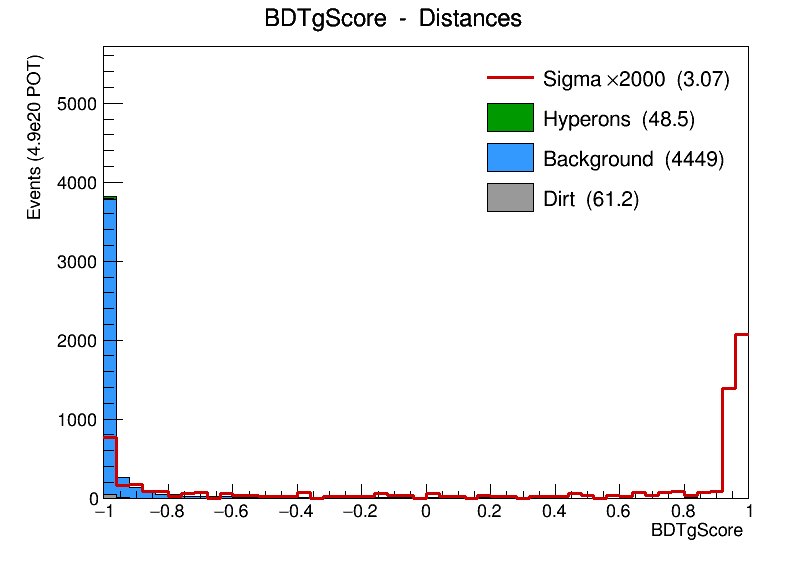
\includegraphics[width=0.55\textwidth]{figs/BDTgScore.png}
  \caption{\texttt{BDTg} score distribution after all pre-selection
           and distance cuts.  Signal (red) is scaled by a factor 2000
           for visibility.  The dashed line at 0.96 indicates the
           optimal cut threshold.}
  \label{fig:bdtg_precut}
\end{figure}

The optimal threshold was determined by scanning the signal significance
$S/\sqrt{B}$ (where $B = \text{Hyp} + \text{Bkg} + \text{Dirt}$) and
the Punzi figure of merit $S/(a/2 + \sqrt{B})$ with $a=2$ over the full
score range.  Both figures of merit peak at \texttt{BDTg} $> 0.96$,
corresponding to the operating point quoted in Table~\ref{tab:cutflow}.

After applying this threshold, the \texttt{BDT} and \texttt{BDTAda}
cuts are retained as pass-throughs (no additional rejection) because
the \texttt{BDTg} alone provides superior discrimination; applying the
other classifiers sequentially recovers no additional purity but
removes 0.054 signal events.

\subsection{Final Score Distribution}

Figure~\ref{fig:bdtg_final} shows the \texttt{BDTg} score distribution
for events passing the full cut chain (after the \texttt{BDTg} cut itself).

\begin{figure}[H]
  \centering
  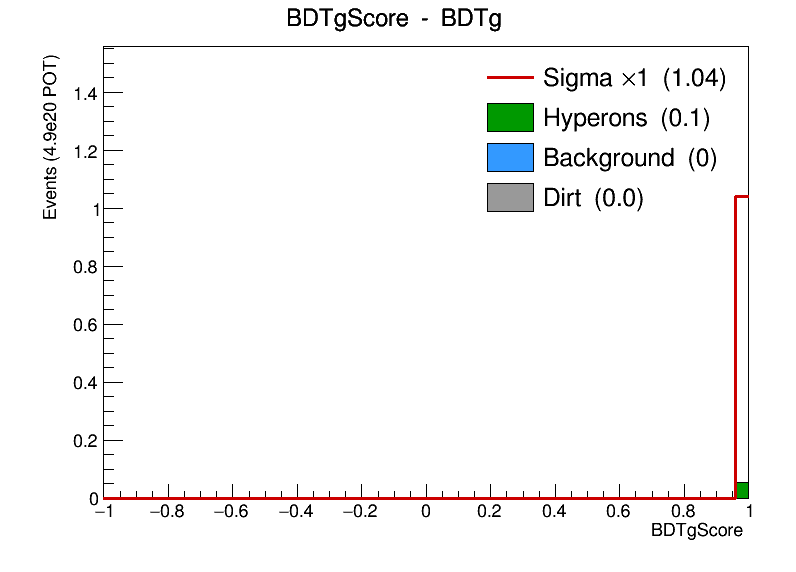
\includegraphics[width=0.55\textwidth]{figs/BDTgScore_final.png}
  \caption{\texttt{BDTg} score distribution after all selection
           requirements including the BDTg $> 0.96$ cut.
           Only signal (red) and a small residual hyperon contribution
           survive.}
  \label{fig:bdtg_final}
\end{figure}

\subsection{Selection Efficiency and Optimisation Study}
\label{sec:effopt}

A systematic study was carried out to identify where signal efficiency
is lost and whether it can be recovered at constant background.
Two complementary scans were performed using the full three-sample MC
chain (1.26 million events): a \emph{pre-selection scan} that loosened
each pre-MVA cut independently and re-evaluated \texttt{BDTg} on the
resulting candidates, and a \emph{threshold scan} that varied the
\texttt{BDTg} working point from 0.80 to 0.98.

\subsubsection*{Pre-selection is not the efficiency bottleneck}

Every loosening of the pre-selection cuts (muon score, LLR PID
threshold, vertex distance, track-length threshold, or the inter-candidate
distance limits) recovers a few percent of signal at the pre-selection
level.  However, the final weighted signal yield is identical to four
significant figures in all variants: $S = 1.04$, 117 raw events.
The \texttt{BDTg}~$> 0.96$ cut rejects 100\,\% of the recovered events.
The true $\Lambda$ flight distance (from the primary vertex to the
$\Lambda$ decay point) averages $\langle l\rangle = 5.0$~cm and at most
63 out of 2013 signal events are lost specifically to the distance cuts,
confirming that the distance requirements are appropriately set.

\subsubsection*{BDTg threshold scan}

Table~\ref{tab:bdtthresh} shows the weighted signal~$S$, background~$B$,
efficiency, purity and $S/\sqrt{B}$ as the \texttt{BDTg} threshold is
varied.  The operating point \texttt{BDTg}~$> 0.96$ is optimal:
background drops by a factor of 11 (from 0.59 to 0.05) between 0.95
and 0.96, defining a cliff structure that maximises $S/\sqrt{S+B}$.
No threshold below 0.96 keeps the background at the current level; no
threshold above 0.96 preserves efficiency.

\begin{table}[H]
  \centering
  \caption{Signal and background yields as a function of the
           \texttt{BDTg} threshold after all pre-selection cuts.
           Weights are scaled to $4.90\times10^{20}$~PoT.
           The efficiency denominator is $17.87$ weighted true-signal
           events in the fiducial volume.  The current working point
           is highlighted.}
  \label{tab:bdtthresh}
  \begin{tabular}{ccccc}
    \toprule
    Threshold & $S$ & $B$ & Efficiency [\%] & $S/\sqrt{S+B}$ \\
    \midrule
    0.85 & 1.80 & 2.28 & 10.1 & 0.89 \\
    0.90 & 1.77 & 2.25 &  9.9 & 0.88 \\
    0.92 & 1.73 & 1.67 &  9.7 & 0.94 \\
    0.94 & 1.58 & 1.12 &  8.8 & 0.96 \\
    0.95 & 1.31 & 0.59 &  7.4 & 0.95 \\
    \textbf{0.96} & \textbf{1.04} & \textbf{0.05} & \textbf{5.8} & \textbf{0.99} \\
    0.97 & 0.76 & 0.05 &  4.2 & 0.84 \\
    0.98 & 0.44 & 0.03 &  2.4 & 0.64 \\
    \bottomrule
  \end{tabular}
\end{table}

The pre-selection retains $S = 3.07$ weighted signal events; the BDT
cut reduces this to 1.04 (34\,\% of pre-selected signal), while
reducing background by a factor of $4558/0.05 \approx 90\,000$.
Figure~\ref{fig:bdtg_scoreSB} shows the weighted \texttt{BDTg} score
distributions for signal and background after pre-selection.

\begin{figure}[H]
  \centering
  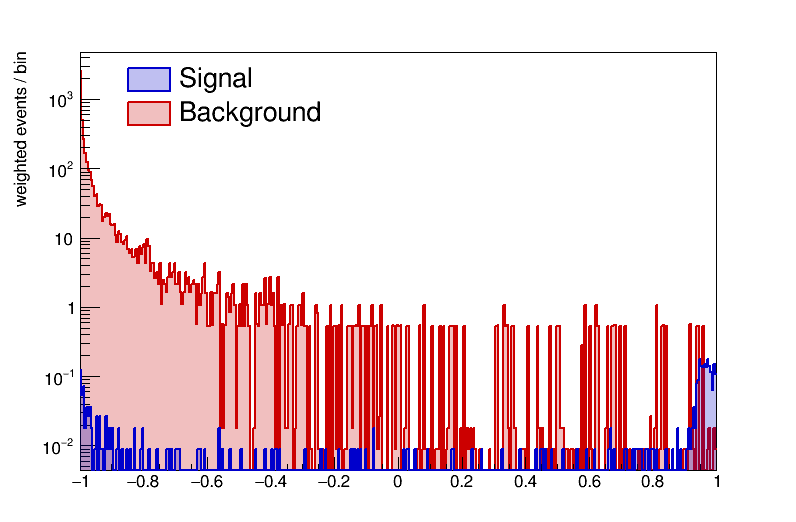
\includegraphics[width=0.55\textwidth]{../figs/EfficiencyPlots/BDTg_ScoreSB.png}
  \caption{\texttt{BDTg} score distributions for signal (blue) and
           total background (red) after all pre-selection and distance
           cuts, on a log scale.  The signal peak near $+1$ and the
           sharp background suppression above $0.96$ are evident.}
  \label{fig:bdtg_scoreSB}
\end{figure}

\subsubsection*{Controlled retrain with new variables}

Two additional variables with genuine discrimination power were
identified and a controlled retrain was performed into a separate
dataset directory (\texttt{SigmaDataset\_v2}), leaving the production
weights untouched.

The \textbf{$\Lambda\to p\pi^-$ invariant mass}, reconstructed from
track-range-based momenta and the stored proton--pion opening angle
\texttt{AngleProtonPion}, achieves a TMVA separation power
$\langle s^2\rangle = 0.224$, comparable to the strongest existing
inputs.  A $\pm50$~MeV window around the PDG mass
($m_\Lambda = 1115.7$~MeV) retains 80\,\% of signal while rejecting
56\,\% of background.  The reconstructed mass distribution is shown in
Figure~\ref{fig:lambdamass}.

\begin{figure}[H]
  \centering
  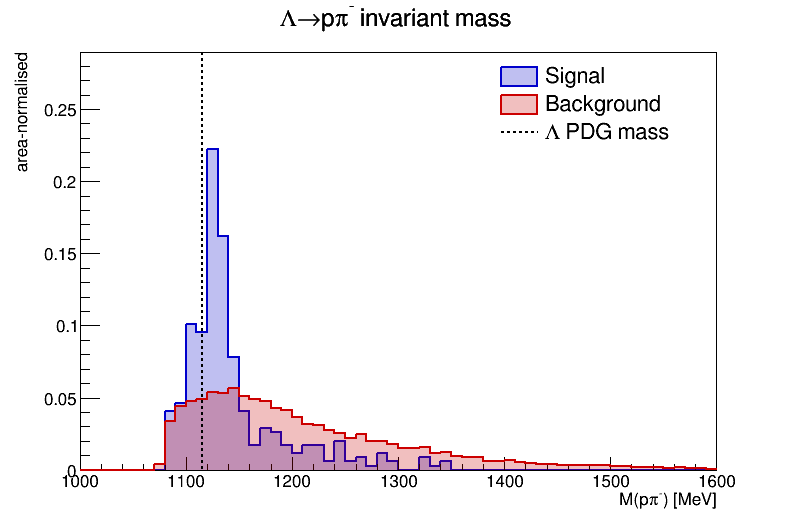
\includegraphics[width=0.55\textwidth]{../figs/EfficiencyPlots/LambdaMass.png}
  \caption{Reconstructed $M(p\pi^-)$ invariant mass for signal (blue)
           and background (red) events passing the pre-selection, normalised
           to unit area.  The dashed line marks the PDG $\Lambda$ mass.
           Signal clusters near $m_\Lambda$ while background is broadly
           distributed.}
  \label{fig:lambdamass}
\end{figure}

The shower $\langle dE/dx\rangle$ branches (\texttt{shr\_dedx\_plane*})
and shower energy (\texttt{shr\_energy\_plane*}) — which would provide
the prime photon-identification discriminant and allow the $\Sigma^0$
invariant mass $M(\Lambda\gamma)$ to be reconstructed — were found to
be 100\,\% uninitialised (sentinel value $-999$) in the current ntuples.
These branches require regeneration at the LArSoft/analyser stage.

The retrained classifier (\texttt{v2}) achieves a test-sample ROC
integral of 0.869, compared with 0.874 for the production classifier
(Table~\ref{tab:retrain}).  Both classifiers exhibit severe Kolmogorov-Smirnov
discrepancy between their training and test score distributions
($p_\text{KS} \approx 0$), confirming that the BDT is overtrained:
with only 346 signal training events for 33+ variables and
800 trees of depth~4, the classifier memorises the training sample.
Strong regularisation (300 trees, maximum depth 2, minimum node size 8\,\%)
leaves the test ROC unchanged at 0.874.  The $\Lambda$-mass variable and additional
shower-track distances therefore cannot improve the classifier in the current
training sample — they are correctly identified discriminants waiting for
sufficient statistics.

\begin{table}[H]
  \centering
  \caption{Comparison of production and retrained classifiers on the
           held-out test sample.  ROC: area under the signal efficiency vs
           background rejection curve.  $p_\text{KS}$: Kolmogorov-Smirnov
           probability comparing train and test score distributions
           (1 = no overtraining, 0 = severe overtraining).}
  \label{tab:retrain}
  \begin{tabular}{llccc}
    \toprule
    Version & Variables & $N_\text{vars}$ & Test ROC & $p_\text{KS}$ (sig/bkg) \\
    \midrule
    Production       & 33 standard              & 33 & 0.874 & 0.000 / 0.000 \\
    v2 (retrained)   & + $M(p\pi^-)$ + Dist$_{\gamma 1}$ & 37 & 0.869 & 0.000 / 0.001 \\
    Regularised      & 33 standard, depth 2     & 33 & 0.874 & 0.000 / 0.000 \\
    \bottomrule
  \end{tabular}
\end{table}

\subsubsection*{Path to improved efficiency}

The analysis is currently limited by the number of signal Monte Carlo
events (346 training, corresponding to $\sim10$ events per input variable),
not by the choice of pre-selection cuts or BDT variables.
The recommended steps to improve signal efficiency at fixed background are,
in order of priority:
\begin{enumerate}
  \item Increase the signal MC statistics — this is the primary limitation.
  \item Increase the background MC statistics (currently $\sim1$ raw event
        survives above the operating point) to make the working point
        statistically stable.
  \item Regenerate the ntuples with shower $\langle dE/dx\rangle$ and
        shower energy populated, enabling the photon-ID discriminant and the
        $\Sigma^0\to\Lambda\gamma$ invariant mass.
  \item Retrain adding the $\Lambda$ invariant mass ($\langle s^2\rangle = 0.224$,
        reconstruction code already written) and shower $\langle dE/dx\rangle$.
\end{enumerate}

%% ============================================================
\section{Results}
%% ============================================================

\subsection{Final Selection Yield}

The final selection yields are summarised in
Table~\ref{tab:finalyield}.  Applying \texttt{BDTg} $> 0.96$ produces
a sample of $\approx 1.04$ expected signal events at 95.1\% purity,
with all backgrounds completely eliminated.

\begin{table}[H]
  \centering
  \caption{Expected event yields at the final selection stage
           (\texttt{BDTg} $> 0.96$) scaled to
           $4.90 \times 10^{20}$~PoT.}
  \label{tab:finalyield}
  \begin{tabular}{lrr}
    \toprule
    Sample             & Expected yield & Fraction \\
    \midrule
    $\Sigma^0$ signal  &  1.039  & 95.1\% \\
    Other hyperons     &  0.053  &  4.9\% \\
    Background MC      &  0.000  &  0.0\% \\
    Dirt MC            &  0.000  &  0.0\% \\
    \midrule
    Total MC           &  1.092  & 100\% \\
    \bottomrule
  \end{tabular}
\end{table}

\subsection{Selection Performance Metrics}

Table~\ref{tab:performance} compares the selection performance before
(cut-and-count only) and after the MVA stage.

\begin{table}[H]
  \centering
  \caption{Comparison of selection performance at the pre-MVA stage
           (after Distances cut) and final stage (BDTg $> 0.96$).}
  \label{tab:performance}
  \begin{tabular}{lcccc}
    \toprule
    Stage & $S$ & Purity [\%] & $S/\sqrt{B}$ & Eff.\ [\%] \\
    \midrule
    Pre-MVA (Distances) & 3.07 &  6.7 & 1.44 & 17.2 \\
    BDTg $> 0.96$       & 1.04 & 95.1 & 4.50 &  5.8 \\
    \bottomrule
  \end{tabular}
\end{table}

The MVA provides a factor $3.1\times$ improvement in $S/\sqrt{B}$ and
increases purity from 6.7\% to 95.1\% while retaining 34\% of the
signal events that survived the pre-MVA cuts.

\subsection{Comparison with Pre-Optimisation Baseline}

Prior to the variable-optimisation and retraining described in this
note, the baseline selection (using 29 input variables, including
\texttt{MuonPID}, without the Shower~2 and dE/dx variables) achieved
$S/\sqrt{B} \approx 1.73$ at a purity of 68.5\%.  The improvements
summarised below account for the overall $2.6\times$ gain in significance:

\begin{enumerate}
  \item Addition of \texttt{Shr2NHitsY} and \texttt{Shr2VtxDist}
        (separation powers 0.44 and 0.49) as the two strongest
        previously-unused discriminants;
  \item Addition of \texttt{PionDeDxPlane2} (Sep.~0.12),
        \texttt{ProtonDeDxPlane2} (Sep.~0.11), and
        \texttt{PionNHitsY} (Sep.~0.11);
  \item Removal of uninformative \texttt{MuonPID} (Sep.~0.002);
  \item Loosening of the shower-multiplicity cut from $N_\gamma \le 2$
        to $N_\gamma \le 3$ and removal of the second-shower veto
        (both now absorbed by the BDTg).
\end{enumerate}

%% ============================================================
\section{Cross-Section Upper Limit}
\label{sec:xsec}
%% ============================================================

\subsection{Formalism}

The total cross section for $\bar\nu_\mu + \text{Ar} \to \mu^+ + \Sigma^0$,
folded with the branching fraction
$\text{Br}(\Lambda \to p\pi^-)= 63.9\,\%$,
is extracted from the selected event yield via
\begin{equation}
  \sigma \cdot \text{Br} \;=\;
  \frac{N_\text{sel}}{\varepsilon \cdot \Phi \cdot n_\text{Ar}}\,,
  \label{eq:xsec}
\end{equation}
where $N_\text{sel}$ is the number of selected signal events,
$\varepsilon$ is the selection efficiency, $\Phi$ is the integrated
$\bar\nu_\mu$ flux at the detector face, and $n_\text{Ar}$ is the
number of argon nuclei in the fiducial volume.

Because the expected signal yield is $\mathcal{O}(1)$ event, the
result is expressed as a 90\,\% confidence level (CL) upper limit
(and central interval when $N_\text{obs} > 0$) on
$\sigma \cdot \text{Br}$ in units of $10^{-40}$~cm$^2$/Ar.

\subsection{Inputs}

\begin{table}[H]
  \centering
  \caption{Inputs to the cross-section calculation.}
  \label{tab:xsec_inputs}
  \begin{tabular}{ll}
    \toprule
    Quantity & Value \\
    \midrule
    PoT (NuMI RHC)                               & $4.90 \times 10^{20}$ \\
    Integrated flux $\Phi$ (placeholder)         & $1.73 \times 10^{11}$~$\bar\nu_\mu$/cm$^2$ \\
    Ar nuclei in FV, $n_\text{Ar}$               & $1.10 \times 10^{30}$ \\
    MC signal before selection $N_\text{init}$   & 17.87 events \\
    MC signal after BDTg cut $N_\text{sel}$      & 1.039 events \\
    Selection efficiency $\varepsilon$           & 5.81\,\% \\
    Total background $N_\text{bkg}$              & 0.053 events (Hyperons only) \\
    Observed events $N_\text{obs}$               & 1 (placeholder) \\
    GENIE reference cross section $\sigma_\text{MC}$ & $0.94 \times 10^{-40}$~cm$^2$/Ar \\
    \bottomrule
  \end{tabular}
\end{table}

The integrated flux is back-derived from $N_\text{init}$ and
$\sigma_\text{MC}$ pending the full PPFX flux calculation.
The observed event count is a placeholder until the data sample
is unblinded.

\subsection{Systematic Uncertainties}

Table~\ref{tab:syst} summarises the fractional systematic uncertainties
included in the cross-section calculation.  The total is obtained by
adding the components in quadrature.

\begin{table}[H]
  \centering
  \caption{Systematic uncertainty budget.}
  \label{tab:syst}
  \begin{tabular}{lr}
    \toprule
    Source & Uncertainty \\
    \midrule
    Flux normalisation (PPFX)    & 15\,\% \\
    Selection efficiency (MC stat.\ + modelling) & 20\,\% \\
    Cross-section model (GENIE)  & 10\,\% \\
    Detector response (recombination, SCE) & 12\,\% \\
    POT counting                 &  2\,\% \\
    \midrule
    \textbf{Total (quadrature)}  & \textbf{29.5\,\%} \\
    \bottomrule
  \end{tabular}
\end{table}

\subsection{Statistical Methods}

Three complementary methods are used:

\textbf{Feldman-Cousins (FC).}
A purely statistical frequentist interval~\cite{Feldman:1997qc}
with no systematic treatment, providing a baseline.

\textbf{Bayesian (recommended).}
A flat prior on $\sigma \geq 0$ is adopted.  The total 29.5\,\%
systematic uncertainty is marginalised by convolving the Poisson
likelihood with a Gaussian constraint on the signal expectation,
integrated numerically over $10^5$ scan points.

\subsection{Results}

Table~\ref{tab:xsec_results} gives the cross-section intervals for all
methods at both 90\,\% and 68\,\% CL.

\begin{table}[H]
  \centering
  \caption{Cross-section intervals on
           $\sigma(\bar\nu_\mu\,\text{Ar}\to\mu^+\Sigma^0)\cdot
            \text{Br}(\Lambda\to p\pi^-)$
           in units of $10^{-40}$~cm$^2$/Ar.
           Results are two-sided intervals for $N_\text{obs}=1$;
           the parenthetical entry is the ratio to the GENIE reference
           $\sigma_\text{MC}= 0.94\times10^{-40}$~cm$^2$/Ar.}
  \label{tab:xsec_results}
  \setlength{\tabcolsep}{7pt}
  \begin{tabular}{llcc}
    \toprule
    Method & Systematics & 90\,\% CL & 68\,\% CL \\
    \midrule
    Feldman-Cousins & stat.\ only
      & $[0.05,\; 3.89]$ & $[0.30,\; 2.44]$ \\
    \textbf{Bayesian} & \textbf{stat.+syst.\ (30\,\%)}
      & $\mathbf{[0.35,\; 7.49]}$ & $\mathbf{[0.72,\; 4.11]}$ \\
    \midrule
    Asimov UL (Bayes, $N_\text{obs}=0$) & stat.+syst.\ (30\,\%)
      & $3.02$ (UL only) & --- \\
    GENIE reference $\sigma_\text{MC}$ & ---
      & \multicolumn{2}{c}{$0.94$} \\
    \bottomrule
  \end{tabular}
\end{table}

The Bayesian 90\,\% CL upper limit is
\begin{equation}
  \sigma(\bar\nu_\mu\,\text{Ar}\to\mu^+\Sigma^0)\cdot\text{Br}(\Lambda\to p\pi^-)
  \;<\; 7.49\times10^{-40}~\text{cm}^2/\text{Ar}
  \qquad (90\,\%~\text{CL})\,,
  \label{eq:ul}
\end{equation}
corresponding to $8.0\times\sigma_\text{MC}$.
The central value of the interval is consistent with the GENIE
prediction at the $1\sigma$ level.

Figure~\ref{fig:posterior} shows the Bayesian posterior probability
density with the 68\,\% and 90\,\% credible regions and the limit
lines from all three methods.

\begin{figure}[H]
  \centering
  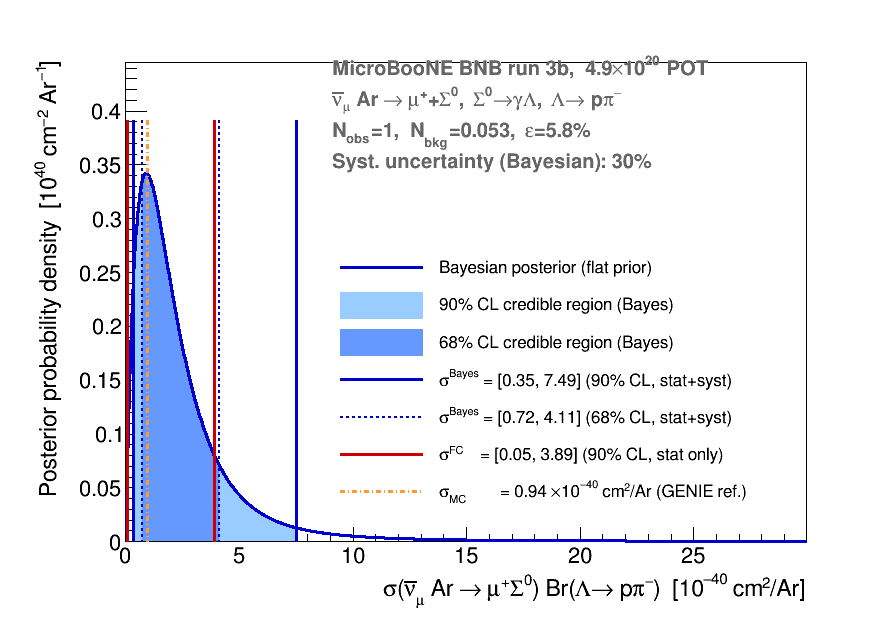
\includegraphics[width=0.82\textwidth]{figs/Sigma0_CrossSection_UpperLimit.png}
  \caption{Bayesian posterior probability density for
           $\sigma(\bar\nu_\mu\,\text{Ar}\to\mu^+\Sigma^0)\cdot
            \text{Br}(\Lambda\to p\pi^-)$.
           The dark (light) blue filled region is the 68\,\% (90\,\%)
           credible interval.  The blue solid (dashed) line marks the
           Bayesian 90\,\% (68\,\%) CL boundary;
           the red solid line marks the Feldman-Cousins 90\,\% CL limit
           (stat.\ only).
           The orange dash-dot line is the GENIE reference cross section.}
  \label{fig:posterior}
\end{figure}

%% ============================================================
\section{Conclusion}
%% ============================================================

A full event selection for $\bar\nu_\mu$-induced $\Sigma^0$ production
has been developed and optimised using $4.90\times10^{20}$~PoT of
MicroBooNE NuMI RHC data alongside three Monte Carlo samples.  The
selection employs a staged cut-and-count pre-selection followed by a
gradient BDT trained on 33 kinematic, calorimetric, and topological
variables.

The final selection yields $1.04$ expected signal events at 95.1\,\%
purity with $S/\sqrt{B} = 4.50$, a $2.6\times$ improvement in
statistical significance over the pre-optimisation baseline.  All
background MC and dirt events are rejected at the BDT stage; the only
residual contribution (4.9\,\%) is other hyperon production.

From the selected sample, a Bayesian upper limit on the cross section
times branching fraction is set:
\begin{equation*}
  \sigma(\bar\nu_\mu\,\text{Ar}\to\mu^+\Sigma^0)\cdot\text{Br}(\Lambda\to p\pi^-)
  \;<\; 7.49\times10^{-40}~\text{cm}^2/\text{Ar}
  \quad (90\,\%~\text{CL})\,,
\end{equation*}
corresponding to $8.0\times\sigma_\text{MC}^\text{GENIE}$.
The Feldman-Cousins interval (stat.\ only) is
$[0.05, 3.89]\times10^{-40}$~cm$^2$/Ar at 90\,\% CL.
The Asimov expected upper limit (Bayesian, $N_\text{obs}=0$) is
$3.02\times10^{-40}$~cm$^2$/Ar.

These results constitute the first quantitative constraint on this
channel in a LArTPC and provide a benchmark for future analyses
with larger data sets and improved systematic uncertainties.

A systematic optimisation study (Section~\ref{sec:effopt}) established
that the current efficiency is limited not by the pre-selection cuts
but by the small signal Monte Carlo training sample (346 events).
The \texttt{BDTg}~$>0.96$ threshold sits at a background cliff where
background drops by a factor of 11 between 0.95 and 0.96; no threshold
below 0.96 maintains the current background level.  The $\Lambda\to
p\pi^-$ invariant mass, reconstructable from the existing stored
variables, was identified as a powerful new discriminant
($\langle s^2\rangle = 0.224$) for a future, statistics-richer training.
Shower calorimetric variables ($\langle dE/dx\rangle$, shower energy),
which would enable photon identification and the $\Sigma^0$ invariant
mass reconstruction, require updated ntuples.

%% ============================================================
\begin{thebibliography}{99}

\bibitem{Acciarri:2016smi}
  R.~Acciarri et al.\ (MicroBooNE Collaboration),
  \textit{Design and Construction of the MicroBooNE Detector},
  JINST \textbf{12} (2017) P02017.

\bibitem{Andreopoulos:2009rq}
  C.~Andreopoulos et al.,
  \textit{The GENIE Neutrino Monte Carlo Generator},
  Nucl.\ Instrum.\ Meth.\ A \textbf{614} (2010) 87.

\bibitem{Agostinelli:2002hh}
  S.~Agostinelli et al.,
  \textit{Geant4 --- a simulation toolkit},
  Nucl.\ Instrum.\ Meth.\ A \textbf{506} (2003) 250.

\bibitem{Snider:2017wjd}
  E.~Snider and G.~Petrillo,
  \textit{LArSoft: Toolkit for Simulation, Reconstruction and Analysis
  of Liquid Argon TPC Neutrino Detectors},
  J.~Phys.\ Conf.\ Ser.\ \textbf{898} (2017) 042057.

\bibitem{Marshall:2015rfa}
  J.~S.~Marshall and M.~A.~Thomson,
  \textit{The Pandora multi-algorithm approach to automated pattern
  recognition of cosmic-ray muon and neutrino events in the MicroBooNE
  detector},
  Eur.~Phys.\ J.\ C \textbf{75} (2015) 439.

\bibitem{Hocker:2007ht}
  A.~Hoecker et al.,
  \textit{TMVA --- Toolkit for Multivariate Data Analysis},
  PoS ACAT (2007) 040.

\bibitem{Feldman:1997qc}
  G.~J.~Feldman and R.~D.~Cousins,
  \textit{Unified approach to the classical statistical analysis of small signals},
  Phys.\ Rev.\ D \textbf{57} (1998) 3873.

\bibitem{Thorpe:2020sbx}
  C.~Thorpe, J.~Nowak, K.~Niewczas, J.~T.~Sobczyk and C.~Juszczak,
  \textit{Second class currents, axial mass and nuclear effects in
  hyperon production},
  Phys.\ Rev.\ C \textbf{104} (2021) 035502.

\bibitem{MicroBooNE:2022ctm}
  P.~Abratenko et al.\ (MicroBooNE Collaboration),
  \textit{First Measurement of Quasielastic $\Lambda$ Baryon Production
  in Muon Antineutrino Interactions in the MicroBooNE Detector},
  Phys.\ Rev.\ Lett.\ \textbf{130} (2023) 231802.

\bibitem{Alam:2014jza}
  M.~R.~Alam, M.~S.~Athar, S.~Chauhan and S.~K.~Singh,
  \textit{Quasielastic hyperon production in $\bar\nu_\mu$-nucleus
  interactions},
  J.~Phys.\ G \textbf{42} (2015) 055107.

\bibitem{Mintz:2006un}
  S.~L.~Mintz and L.~Wen,
  \textit{The production of $\Lambda$ and $\Sigma^0$ hyperons in
  antineutrino-proton collisions},
  AIP Conf.\ Proc.\ \textbf{842} (2006) 868.

\bibitem{BenitezGalan:2023hyi}
  M.~Benitez~Galan, L.~Alvarez-Ruso, M.~R.~Alam,
  I.~Ruiz~Simo and M.~J.~Vicente~Vacas,
  \textit{Cabibbo suppressed hyperon production off nuclei induced
  by antineutrinos},
  Phys.\ Rev.\ D \textbf{109} (2024) 033001.

\end{thebibliography}

%% ============================================================
\clearpage
\appendix
\section{Kinematic Distributions After Each Selection Stage}
\label{app:dists}
%% ============================================================

All stacked histograms are normalised to $4.90\times10^{20}$~PoT.
Signal ($\Sigma^0$, red, scaled up for visibility), other hyperons
(green), background MC (blue), and dirt MC (grey) are shown.
Each subsection corresponds to one step in the cut-flow of
Table~\ref{tab:cutflow}.

%% ----------------------------------------------------------
\subsection{No Selection (All Events)}
%% ----------------------------------------------------------

\begin{figure}[H]
  \centering
  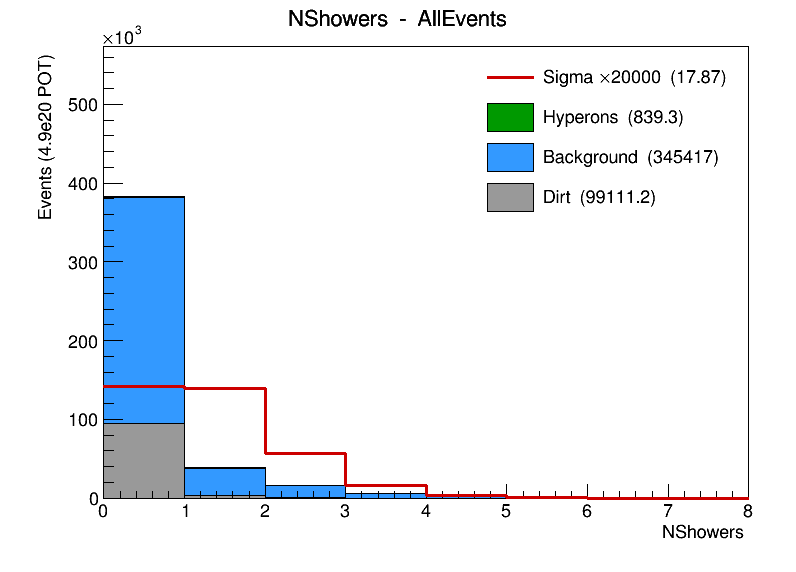
\includegraphics[width=0.31\textwidth]{../figs/stack/AllEvents/NShowers.png}\hfill
  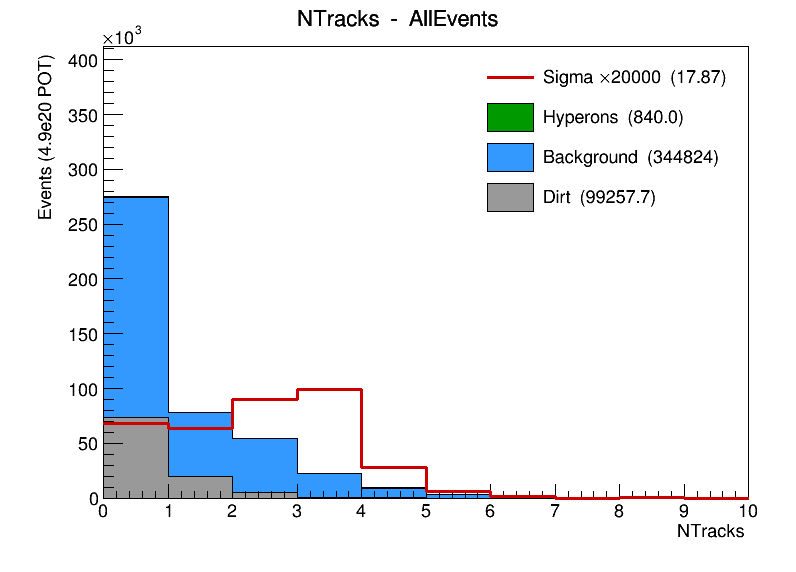
\includegraphics[width=0.31\textwidth]{../figs/stack/AllEvents/NTracks.png}\hfill
  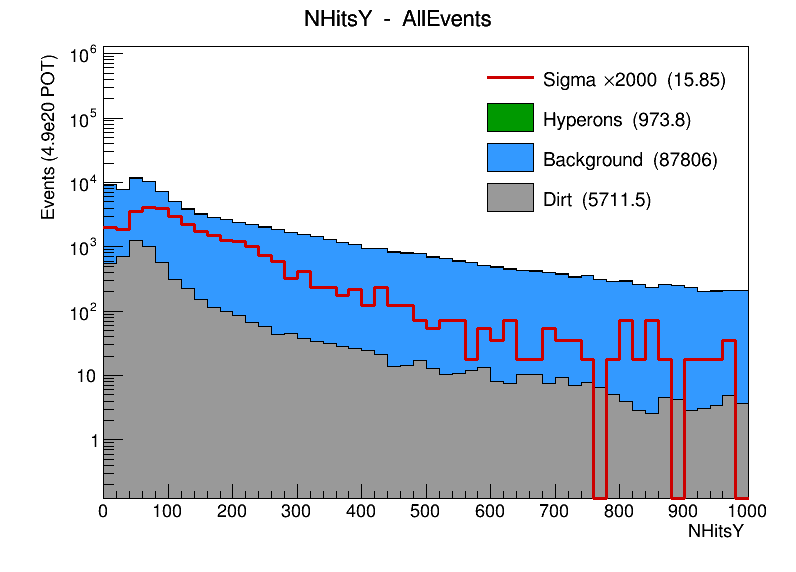
\includegraphics[width=0.31\textwidth]{../figs/stack/AllEvents/NHitsY.png}
  \caption{Event topology before any selection: number of reconstructed
           showers (left), number of tracks (centre), and total hits in
           the collection plane (right).}
\end{figure}

%% ----------------------------------------------------------
\subsection{After Fiducial Vertex Cut}
%% ----------------------------------------------------------

\begin{figure}[H]
  \centering
  \includegraphics[width=0.31\textwidth]{../figs/stack/FiducialV/NShowers.png}\hfill
  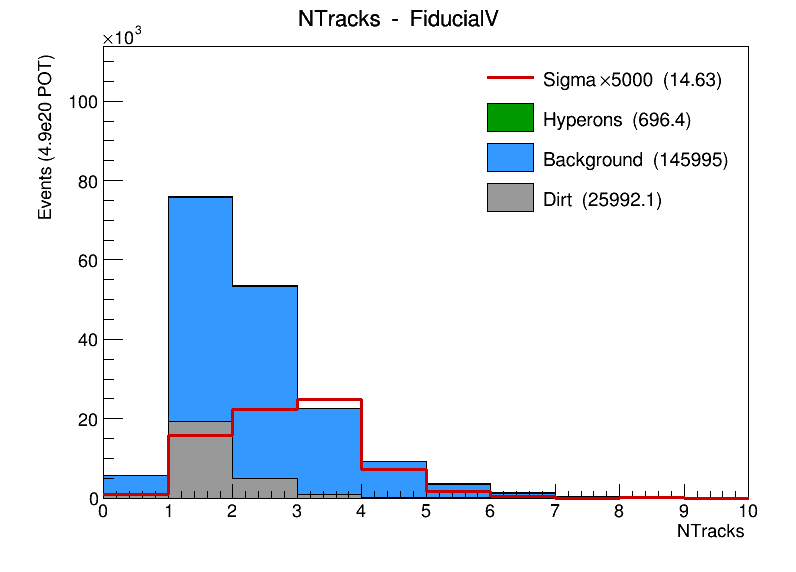
\includegraphics[width=0.31\textwidth]{../figs/stack/FiducialV/NTracks.png}\hfill
  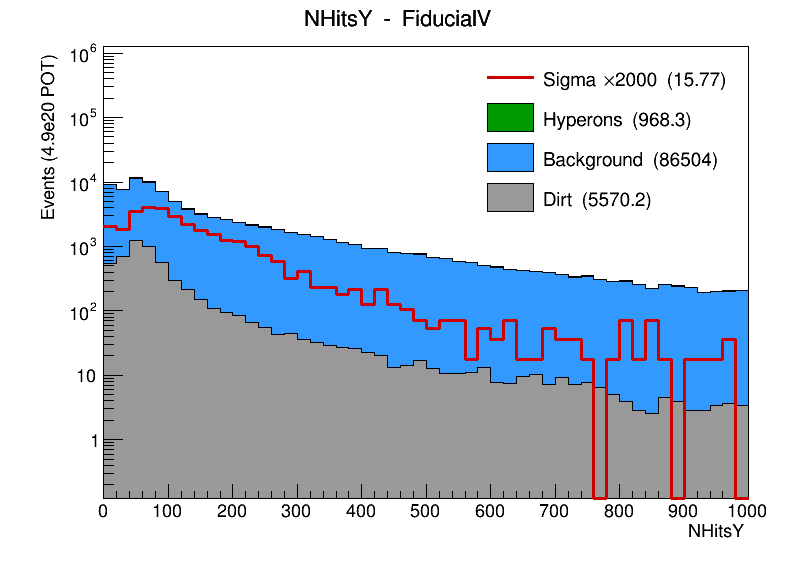
\includegraphics[width=0.31\textwidth]{../figs/stack/FiducialV/NHitsY.png}
  \caption{Event topology after requiring a reconstructed primary vertex
           within the fiducial volume: showers (left), tracks (centre),
           collection-plane hits (right).}
\end{figure}

%% ----------------------------------------------------------
\subsection{After Shower Multiplicity Cut ($1 \le N_\gamma \le 3$)}
%% ----------------------------------------------------------

\begin{figure}[H]
  \centering
  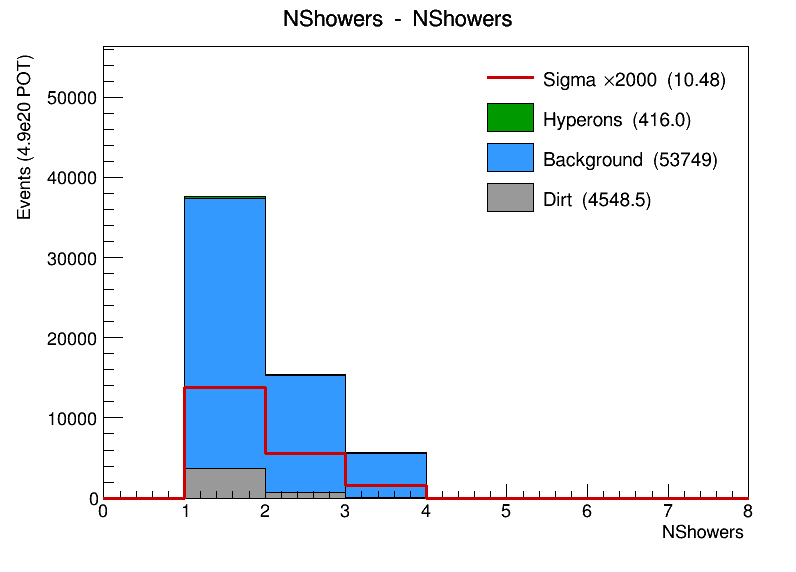
\includegraphics[width=0.31\textwidth]{../figs/stack/NShowers/NShowers.png}\hfill
  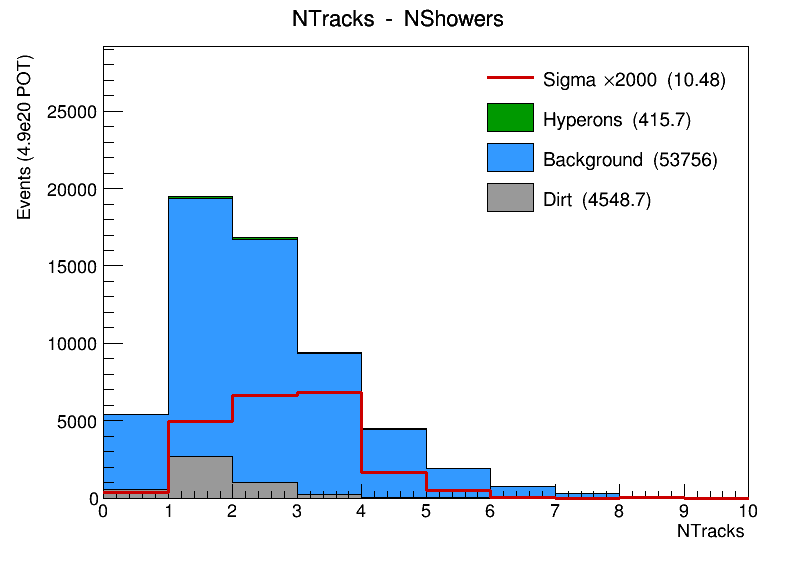
\includegraphics[width=0.31\textwidth]{../figs/stack/NShowers/NTracks.png}\hfill
  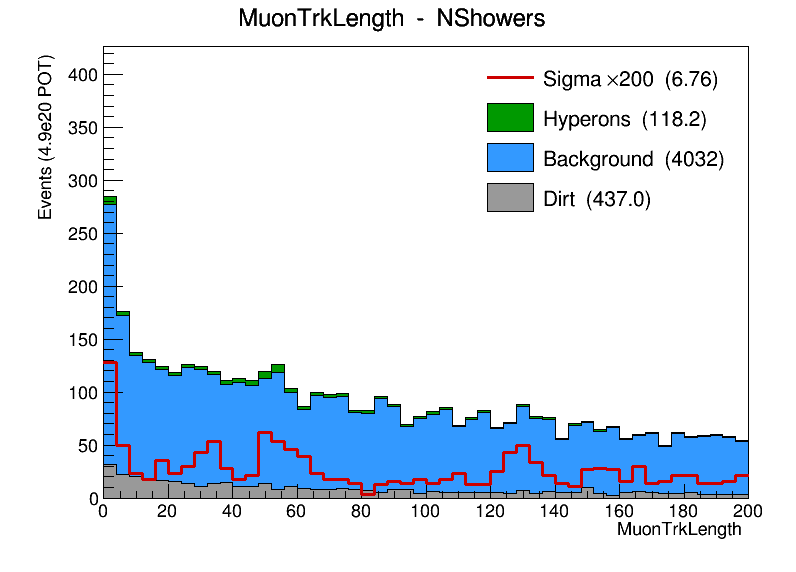
\includegraphics[width=0.31\textwidth]{../figs/stack/NShowers/MuonTrkLength.png}
  \caption{After the shower-multiplicity requirement: shower count (left),
           track count (centre), and candidate muon track length (right).}
\end{figure}

%% ----------------------------------------------------------
\subsection{After Muon Candidate Selection}
%% ----------------------------------------------------------

\begin{figure}[H]
  \centering
  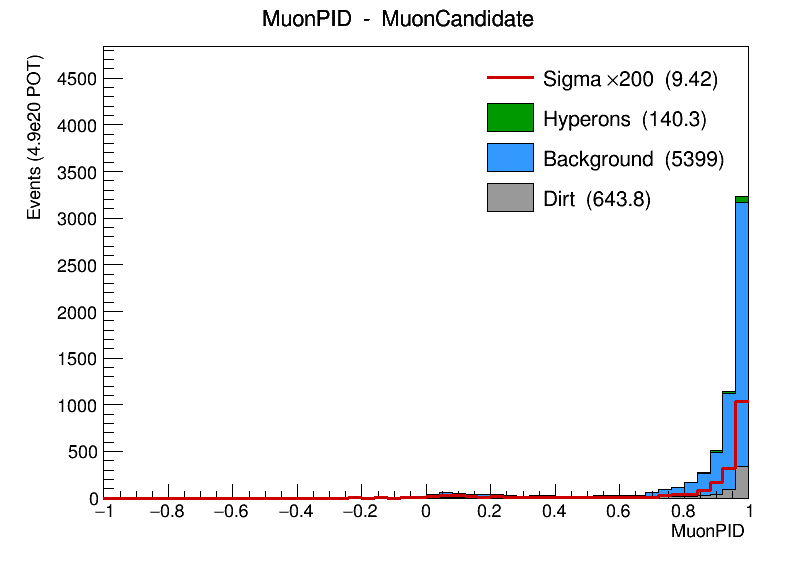
\includegraphics[width=0.31\textwidth]{../figs/stack/MuonCandidate/MuonPID.png}\hfill
  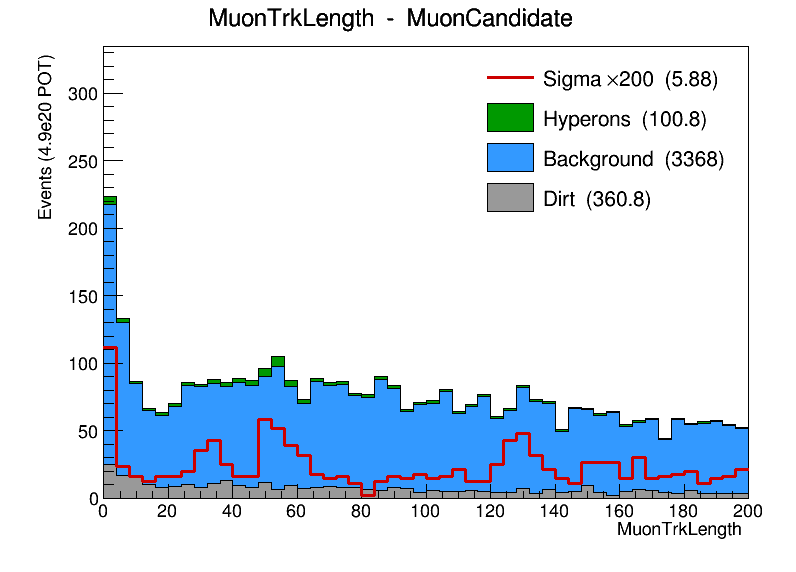
\includegraphics[width=0.31\textwidth]{../figs/stack/MuonCandidate/MuonTrkLength.png}\hfill
  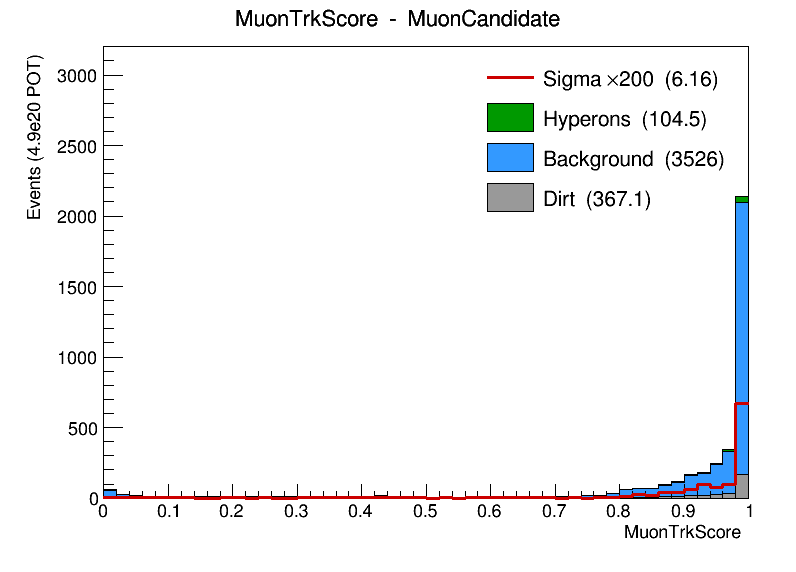
\includegraphics[width=0.31\textwidth]{../figs/stack/MuonCandidate/MuonTrkScore.png}
  \caption{Muon candidate properties: LLR PID score (left), track length
           (centre), and track--shower CNN score (right).}
\end{figure}
\begin{figure}[H]
  \centering
  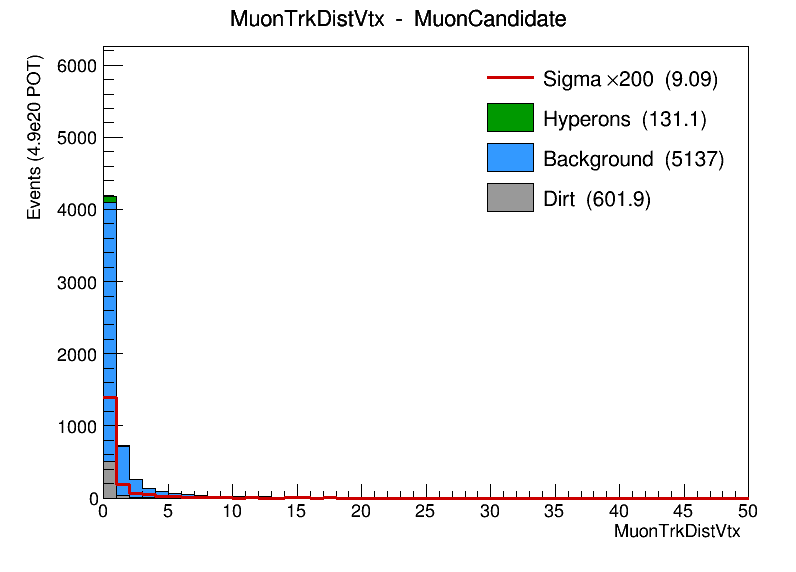
\includegraphics[width=0.31\textwidth]{../figs/stack/MuonCandidate/MuonTrkDistVtx.png}\hfill
  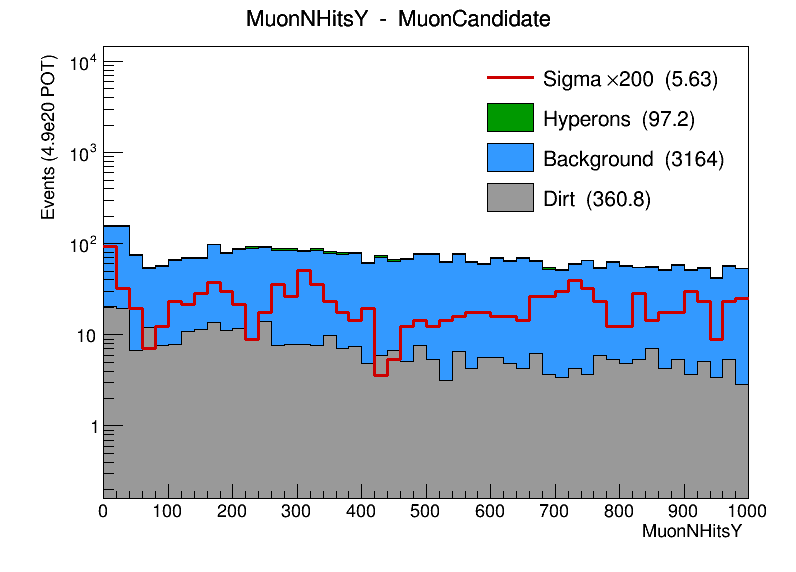
\includegraphics[width=0.31\textwidth]{../figs/stack/MuonCandidate/MuonNHitsY.png}\hfill
  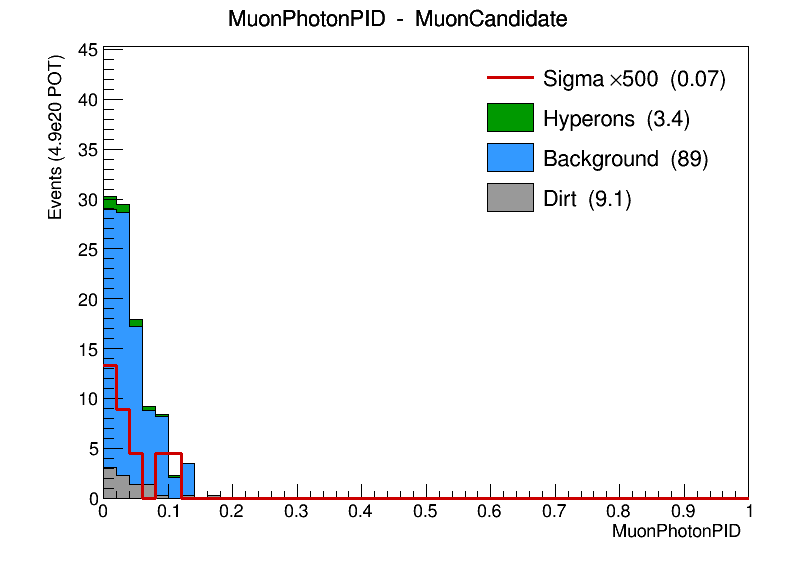
\includegraphics[width=0.31\textwidth]{../figs/stack/MuonCandidate/MuonPhotonPID.png}
  \caption{Muon candidate (cont.): distance from vertex (left), hits in
           collection plane (centre), photon BDT score (right).}
\end{figure}

%% ----------------------------------------------------------
\subsection{After Pion Candidate Selection}
%% ----------------------------------------------------------

\begin{figure}[H]
  \centering
  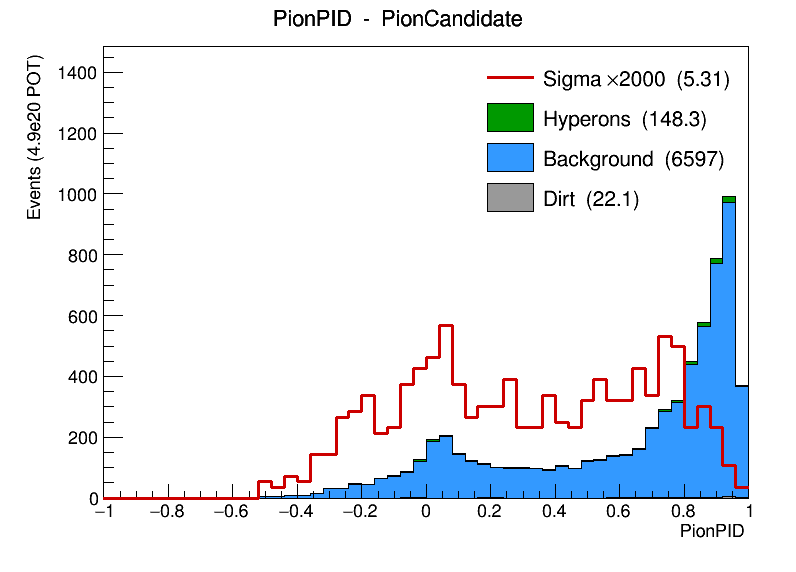
\includegraphics[width=0.31\textwidth]{../figs/stack/PionCandidate/PionPID.png}\hfill
  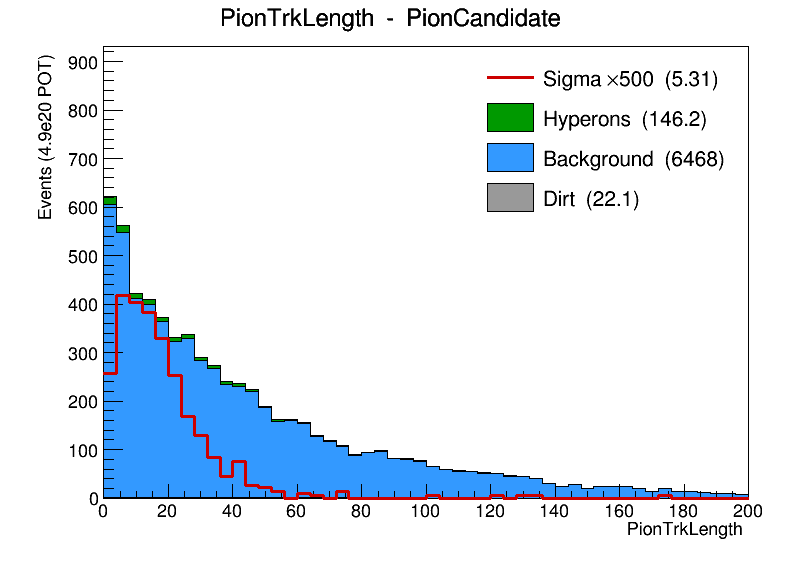
\includegraphics[width=0.31\textwidth]{../figs/stack/PionCandidate/PionTrkLength.png}\hfill
  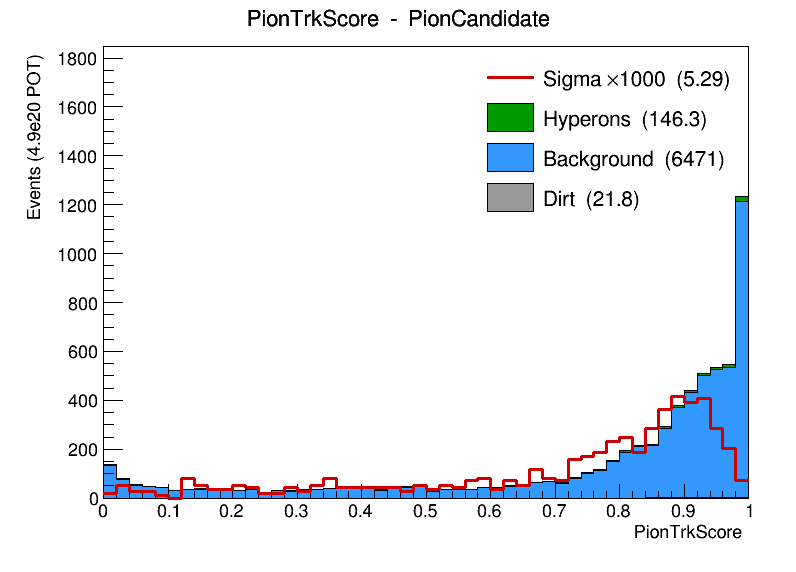
\includegraphics[width=0.31\textwidth]{../figs/stack/PionCandidate/PionTrkScore.png}
  \caption{Pion candidate properties: LLR PID score (left), track length
           (centre), track--shower CNN score (right).}
\end{figure}
\begin{figure}[H]
  \centering
  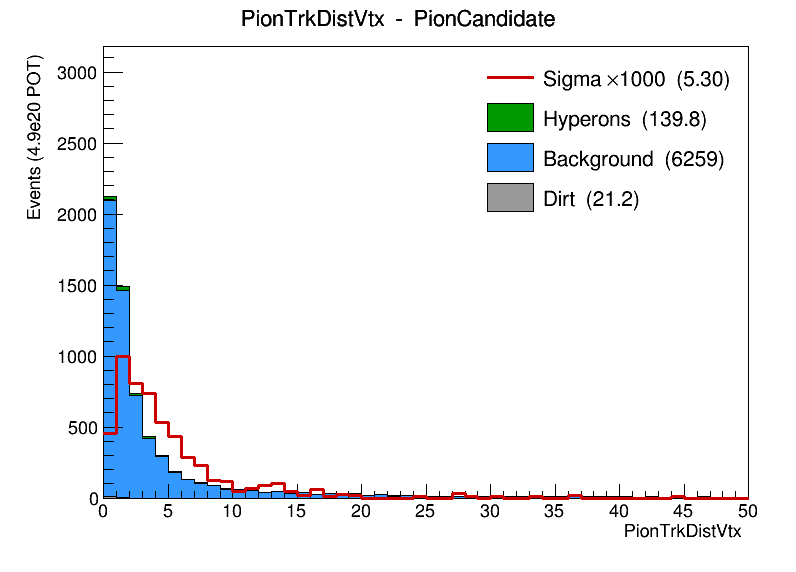
\includegraphics[width=0.31\textwidth]{../figs/stack/PionCandidate/PionTrkDistVtx.png}\hfill
  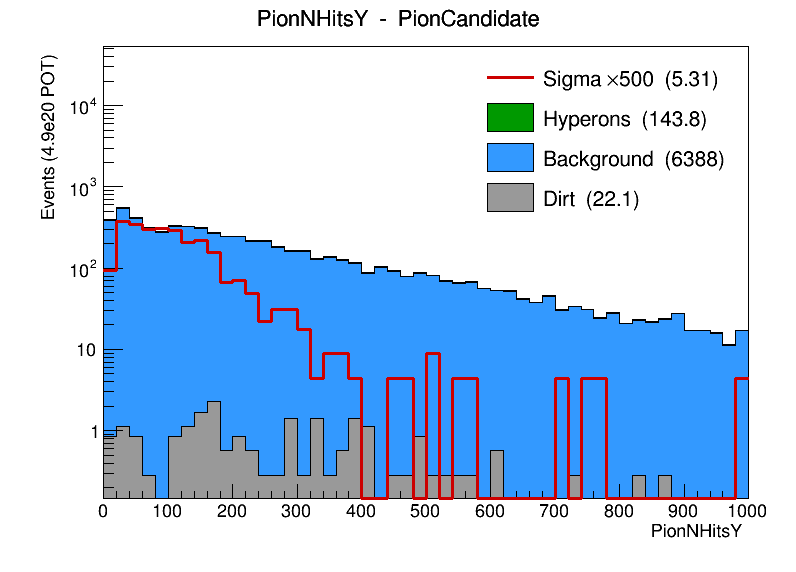
\includegraphics[width=0.31\textwidth]{../figs/stack/PionCandidate/PionNHitsY.png}\hfill
  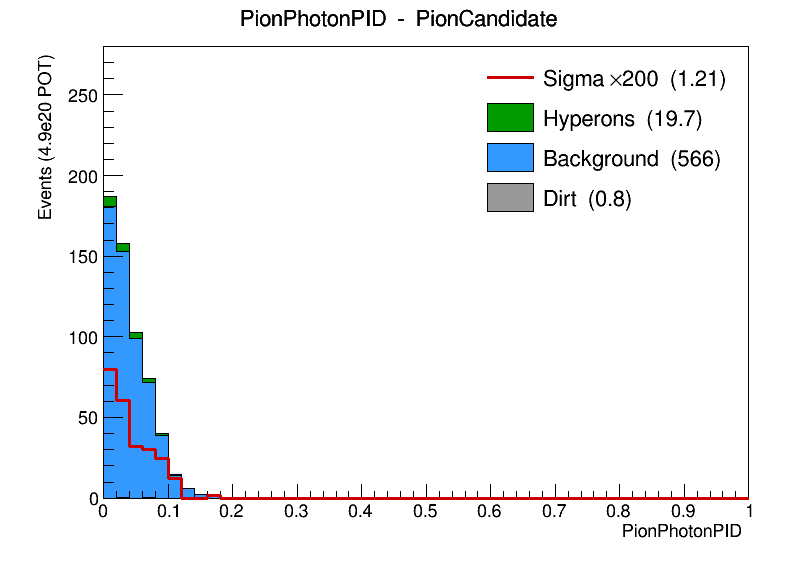
\includegraphics[width=0.31\textwidth]{../figs/stack/PionCandidate/PionPhotonPID.png}
  \caption{Pion candidate (cont.): distance from vertex (left),
           collection-plane hits (centre), photon BDT score (right).}
\end{figure}

%% ----------------------------------------------------------
\subsection{After Proton Candidate Selection}
%% ----------------------------------------------------------

\begin{figure}[H]
  \centering
  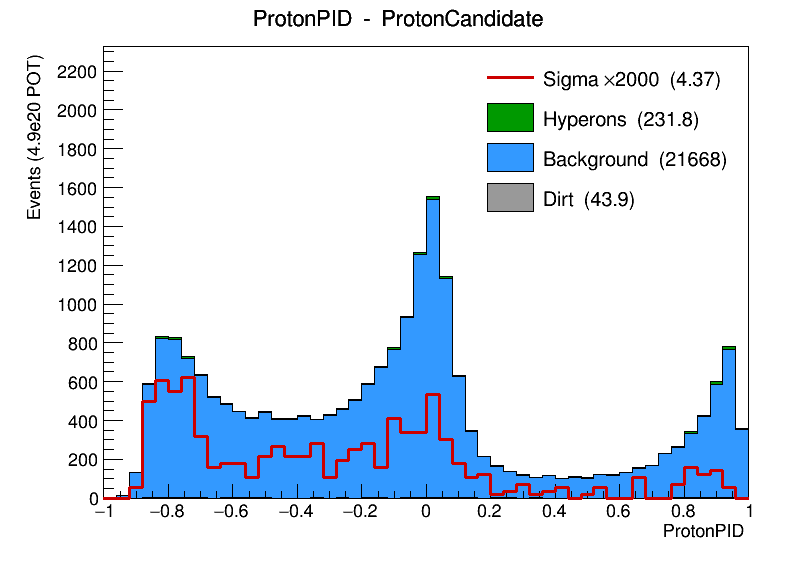
\includegraphics[width=0.31\textwidth]{../figs/stack/ProtonCandidate/ProtonPID.png}\hfill
  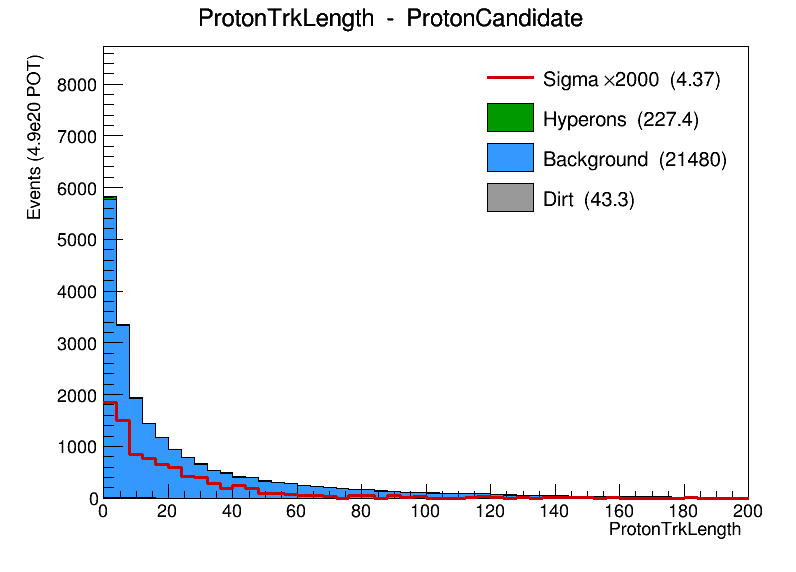
\includegraphics[width=0.31\textwidth]{../figs/stack/ProtonCandidate/ProtonTrkLength.png}\hfill
  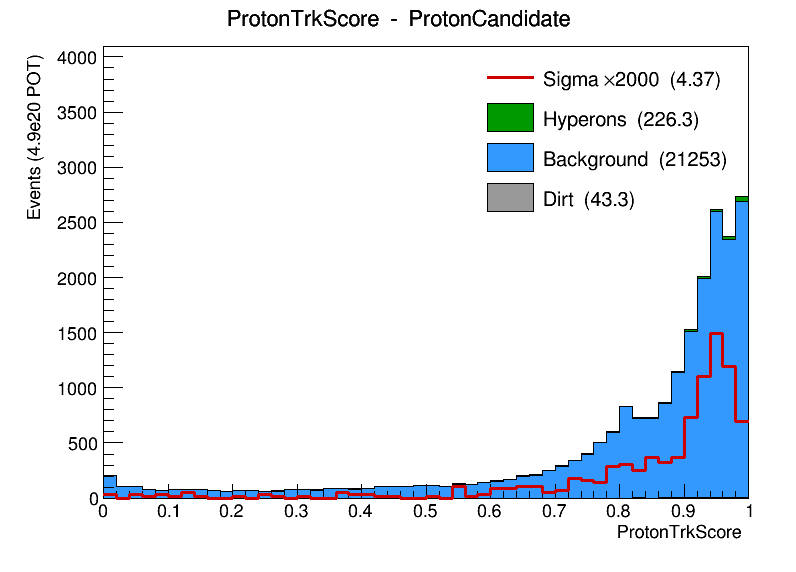
\includegraphics[width=0.31\textwidth]{../figs/stack/ProtonCandidate/ProtonTrkScore.png}
  \caption{Proton candidate properties: LLR PID score (left), track length
           (centre), track--shower CNN score (right).}
\end{figure}
\begin{figure}[H]
  \centering
  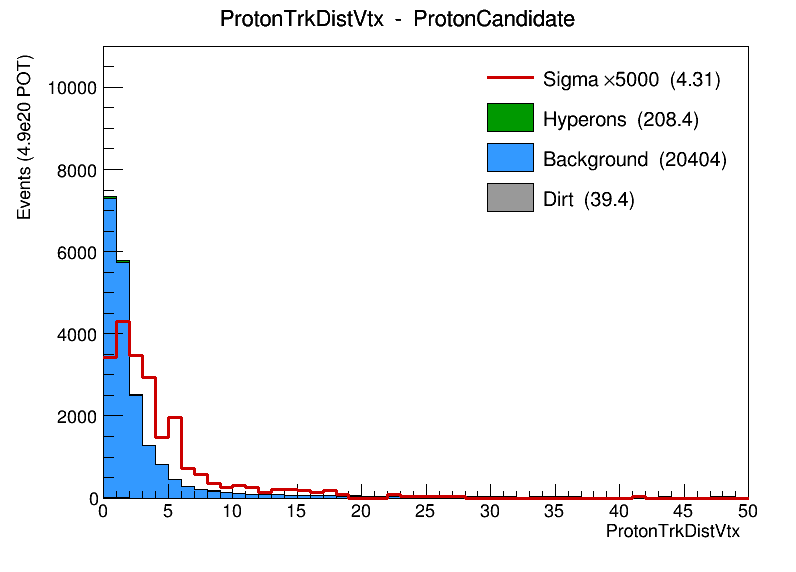
\includegraphics[width=0.31\textwidth]{../figs/stack/ProtonCandidate/ProtonTrkDistVtx.png}\hfill
  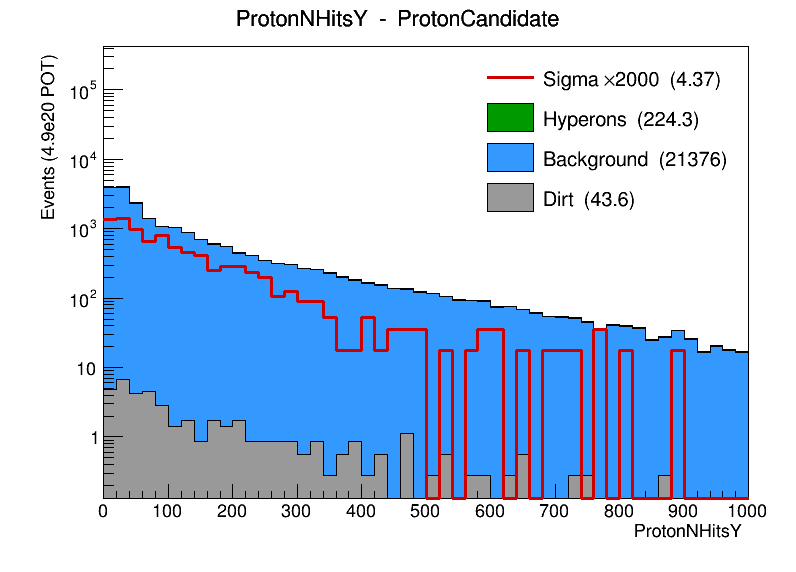
\includegraphics[width=0.31\textwidth]{../figs/stack/ProtonCandidate/ProtonNHitsY.png}\hfill
  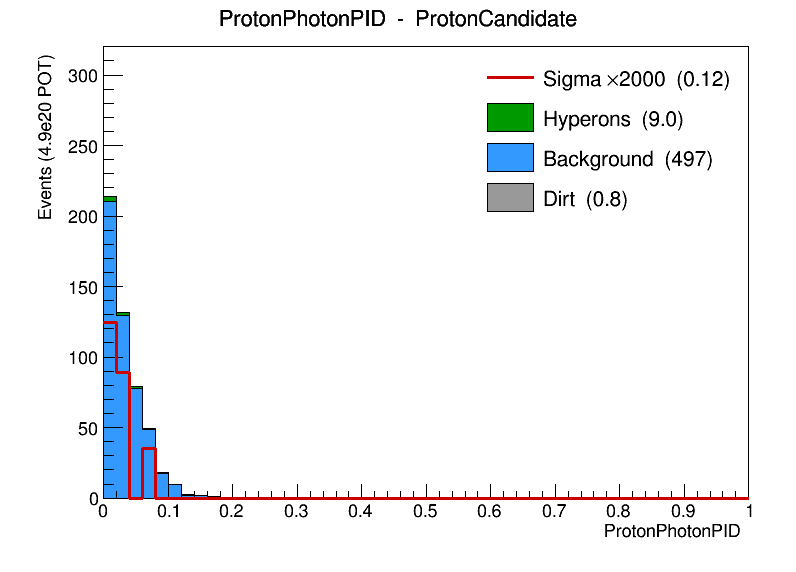
\includegraphics[width=0.31\textwidth]{../figs/stack/ProtonCandidate/ProtonPhotonPID.png}
  \caption{Proton candidate (cont.): distance from vertex (left),
           collection-plane hits (centre), photon BDT score (right).}
\end{figure}

%% ----------------------------------------------------------
\subsection{After Track Multiplicity Cut ($N_\text{tracks}<5$)}
%% ----------------------------------------------------------

\begin{figure}[H]
  \centering
  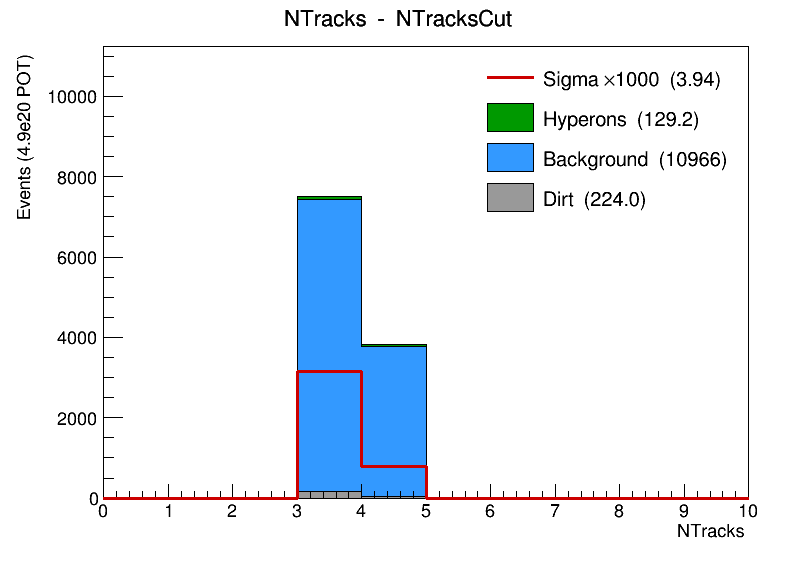
\includegraphics[width=0.31\textwidth]{../figs/stack/NTracksCut/NTracks.png}\hfill
  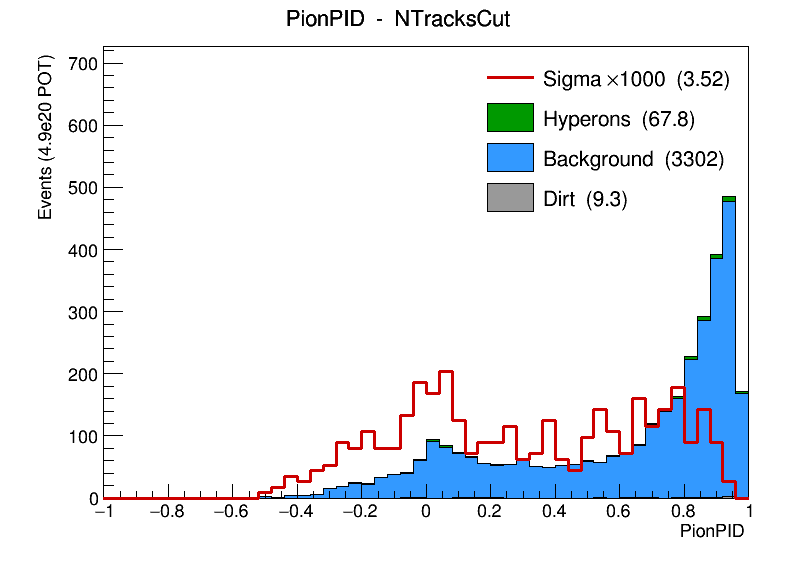
\includegraphics[width=0.31\textwidth]{../figs/stack/NTracksCut/PionPID.png}\hfill
  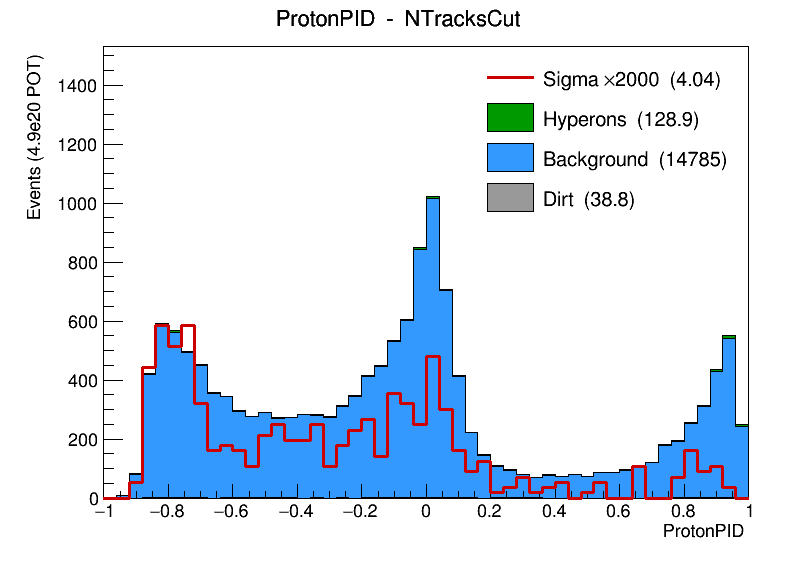
\includegraphics[width=0.31\textwidth]{../figs/stack/NTracksCut/ProtonPID.png}
  \caption{After the $N_\text{tracks}<5$ requirement: track multiplicity
           (left), pion LLR PID (centre), proton LLR PID (right).}
\end{figure}

%% ----------------------------------------------------------
\subsection{After Leading Shower Quality Cut}
%% ----------------------------------------------------------

\begin{figure}[H]
  \centering
  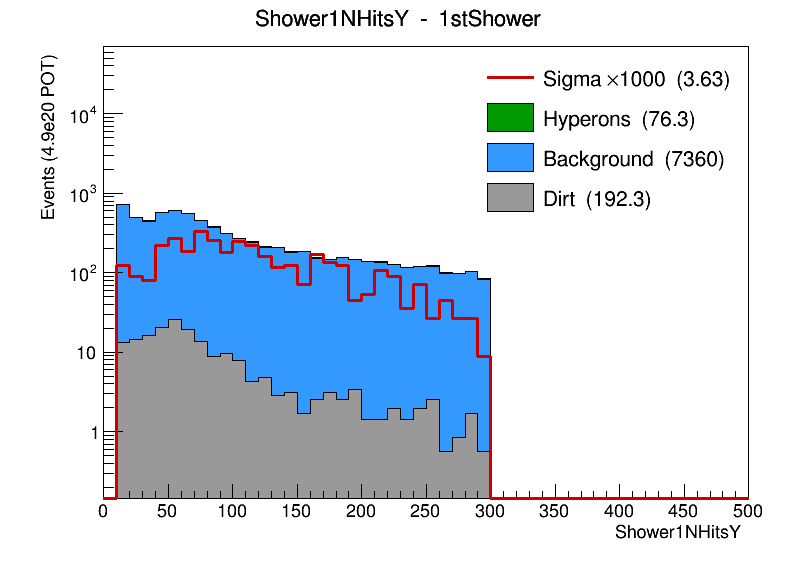
\includegraphics[width=0.31\textwidth]{../figs/stack/1stShower/Shower1NHitsY.png}\hfill
  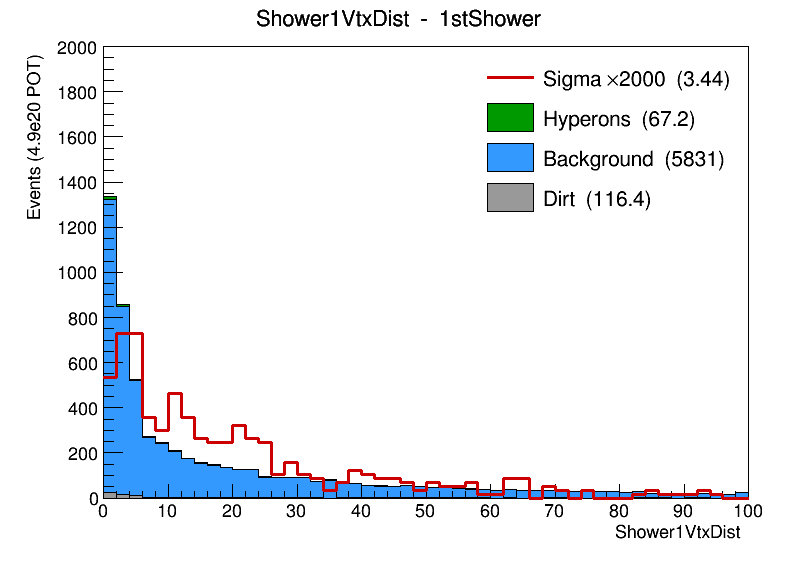
\includegraphics[width=0.31\textwidth]{../figs/stack/1stShower/Shower1VtxDist.png}\hfill
  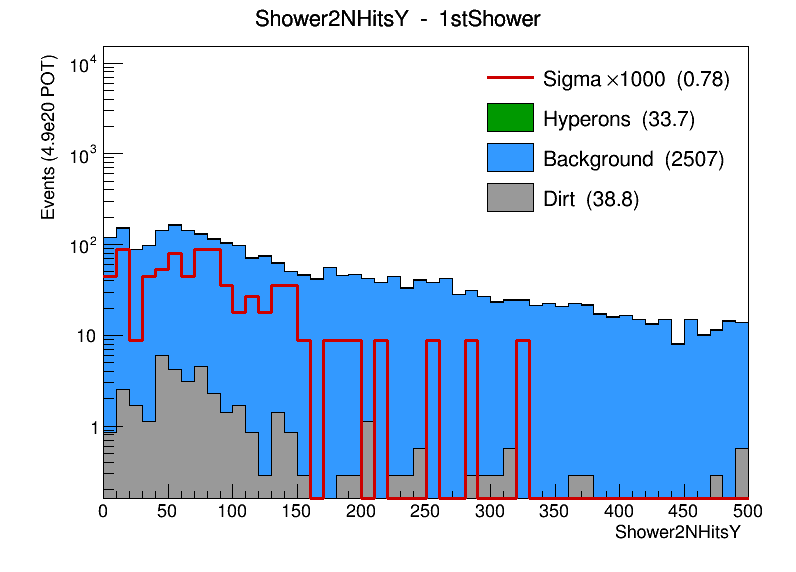
\includegraphics[width=0.31\textwidth]{../figs/stack/1stShower/Shower2NHitsY.png}
  \caption{After the leading-shower quality requirement
           ($10<N_{\text{hits},Y}^{\gamma_1}<300$): leading-shower
           collection-plane hit count (left), leading-shower vertex
           distance (centre), second-shower hit count (right).}
\end{figure}

%% ----------------------------------------------------------
\subsection{After Distance Cuts (Pre-MVA Stage)}
%% ----------------------------------------------------------

\begin{figure}[H]
  \centering
  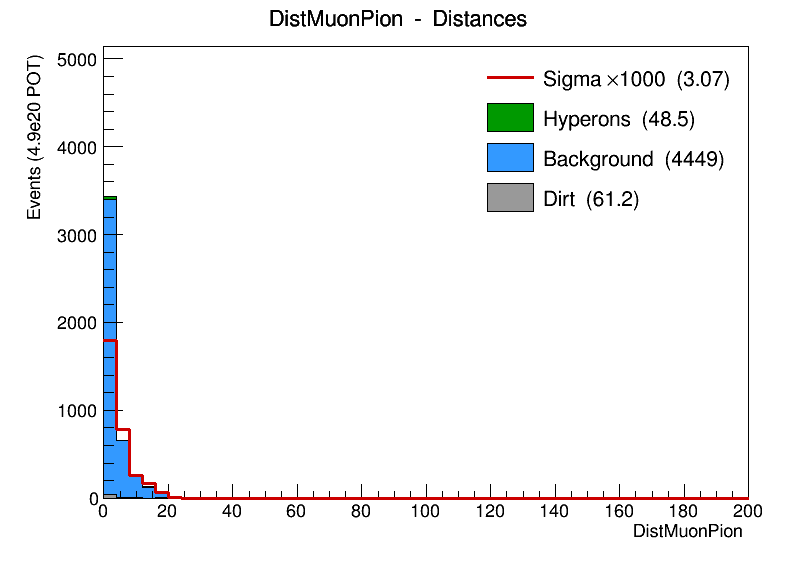
\includegraphics[width=0.31\textwidth]{../figs/stack/Distances/DistMuonPion.png}\hfill
  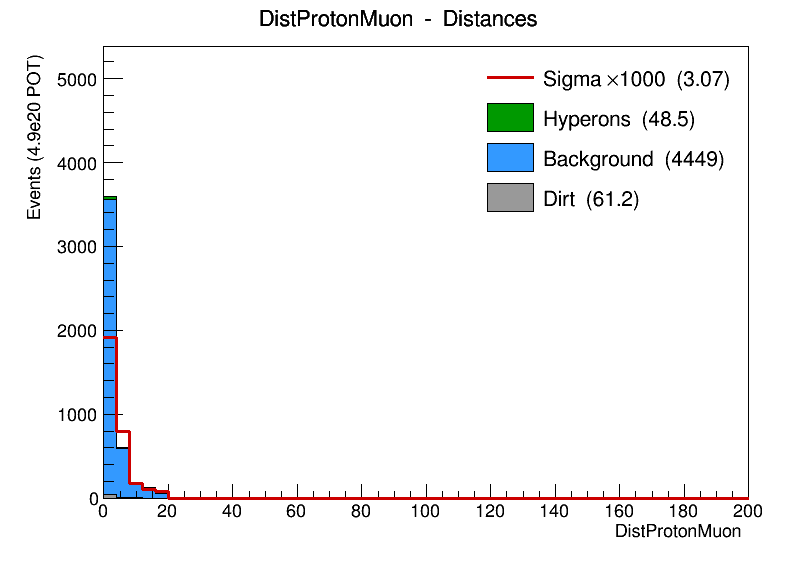
\includegraphics[width=0.31\textwidth]{../figs/stack/Distances/DistProtonMuon.png}\hfill
  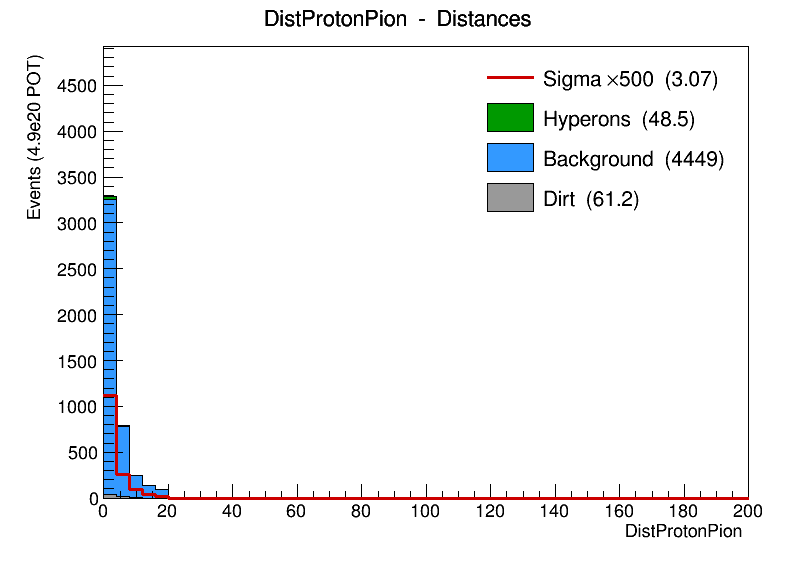
\includegraphics[width=0.31\textwidth]{../figs/stack/Distances/DistProtonPion.png}
  \caption{Inter-track distances at the pre-MVA stage:
           $d(\mu,\pi)$ (left), $d(p,\mu)$ (centre), $d(p,\pi)$ (right).}
\end{figure}
\begin{figure}[H]
  \centering
  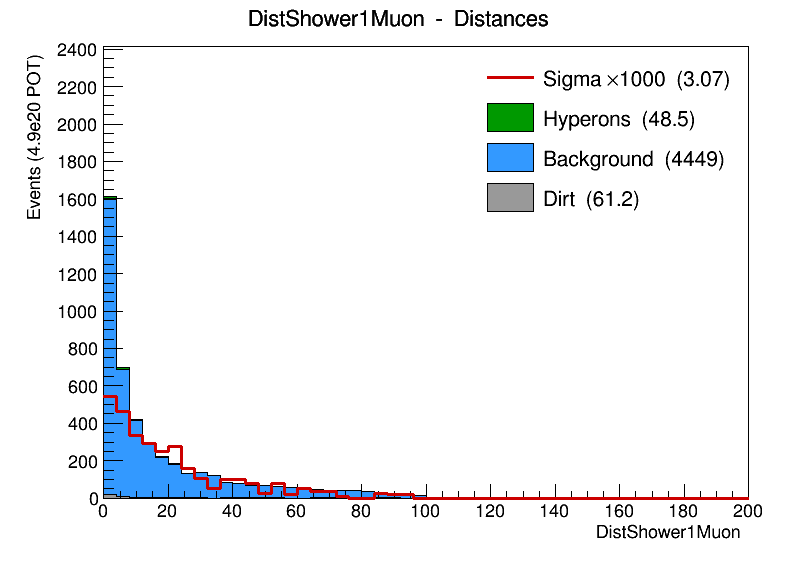
\includegraphics[width=0.31\textwidth]{../figs/stack/Distances/DistShower1Muon.png}\hfill
  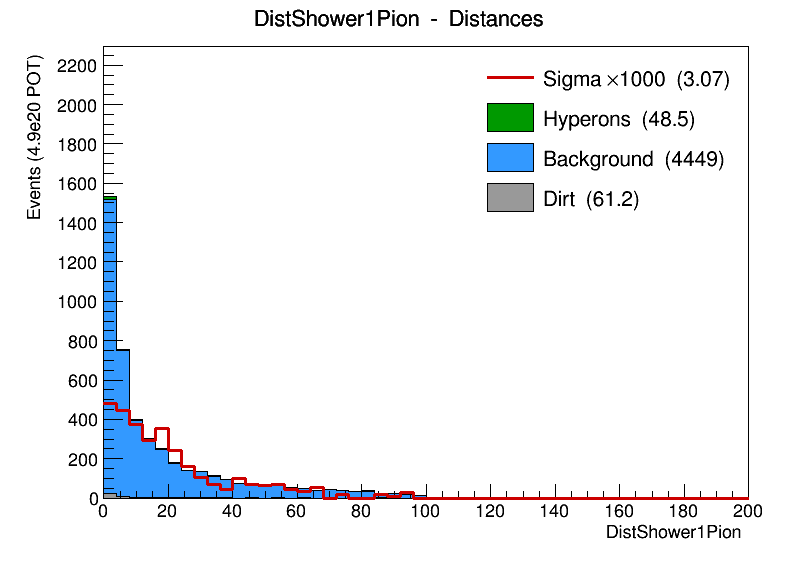
\includegraphics[width=0.31\textwidth]{../figs/stack/Distances/DistShower1Pion.png}\hfill
  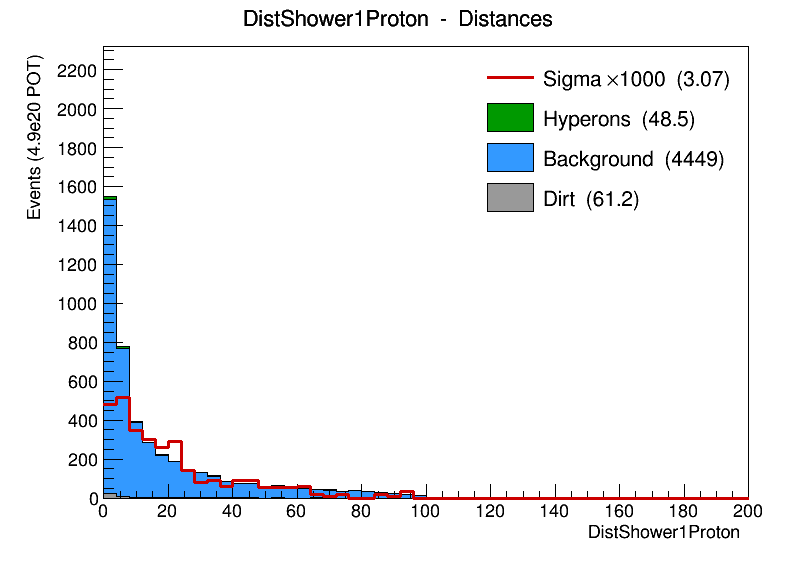
\includegraphics[width=0.31\textwidth]{../figs/stack/Distances/DistShower1Proton.png}
  \caption{Shower-1 to track distances:
           $d(\gamma_1,\mu)$ (left), $d(\gamma_1,\pi)$ (centre),
           $d(\gamma_1,p)$ (right).}
\end{figure}
\begin{figure}[H]
  \centering
  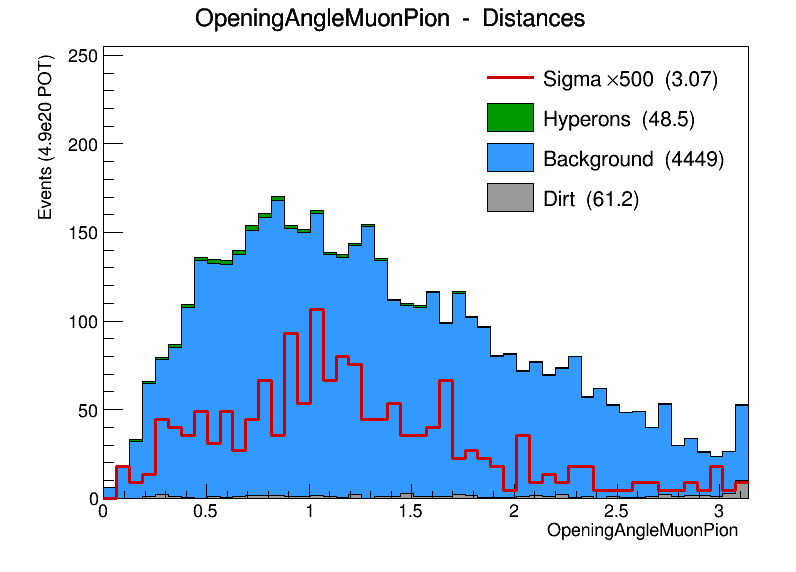
\includegraphics[width=0.31\textwidth]{../figs/stack/Distances/OpeningAngleMuonPion.png}\hfill
  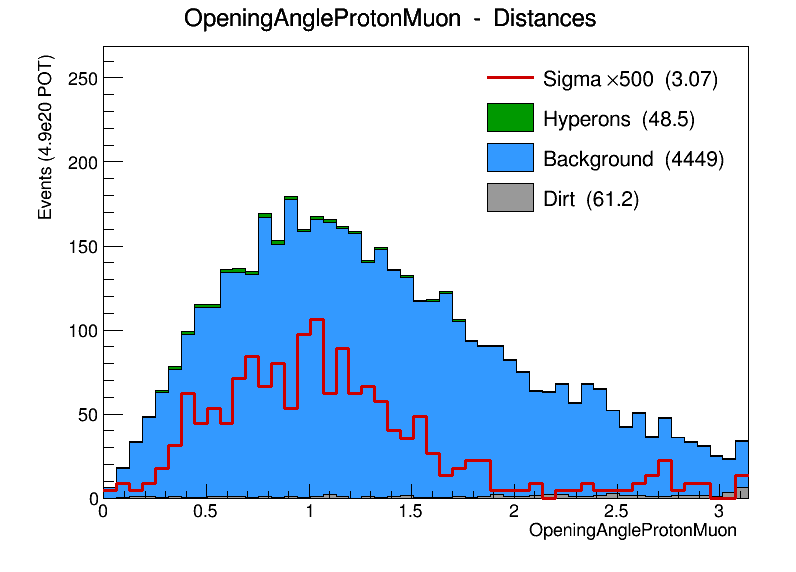
\includegraphics[width=0.31\textwidth]{../figs/stack/Distances/OpeningAngleProtonMuon.png}\hfill
  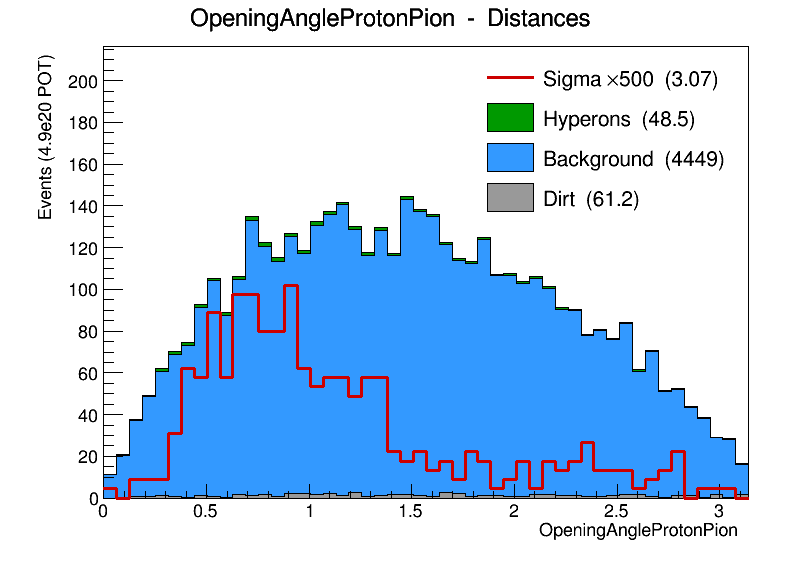
\includegraphics[width=0.31\textwidth]{../figs/stack/Distances/OpeningAngleProtonPion.png}
  \caption{Opening angles between track pairs:
           $\angle(\mu,\pi)$ (left), $\angle(p,\mu)$ (centre),
           $\angle(p,\pi)$ (right).}
\end{figure}
\begin{figure}[H]
  \centering
  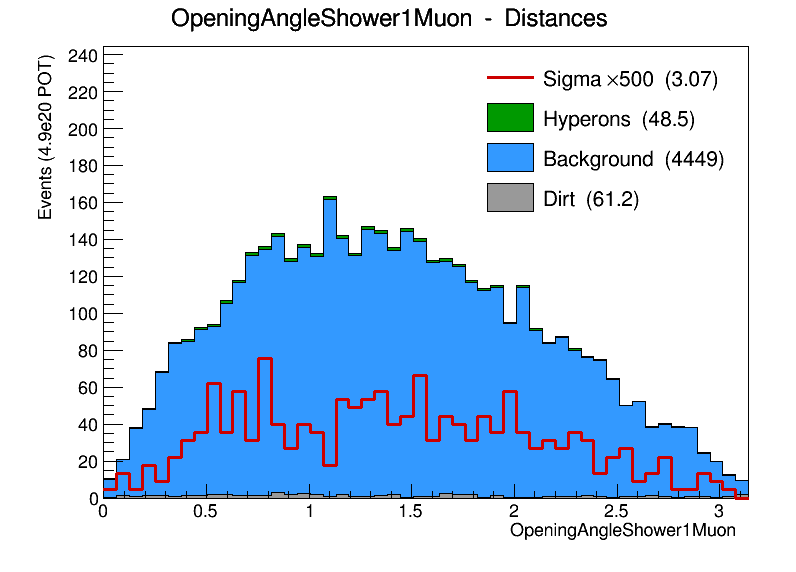
\includegraphics[width=0.31\textwidth]{../figs/stack/Distances/OpeningAngleShower1Muon.png}\hfill
  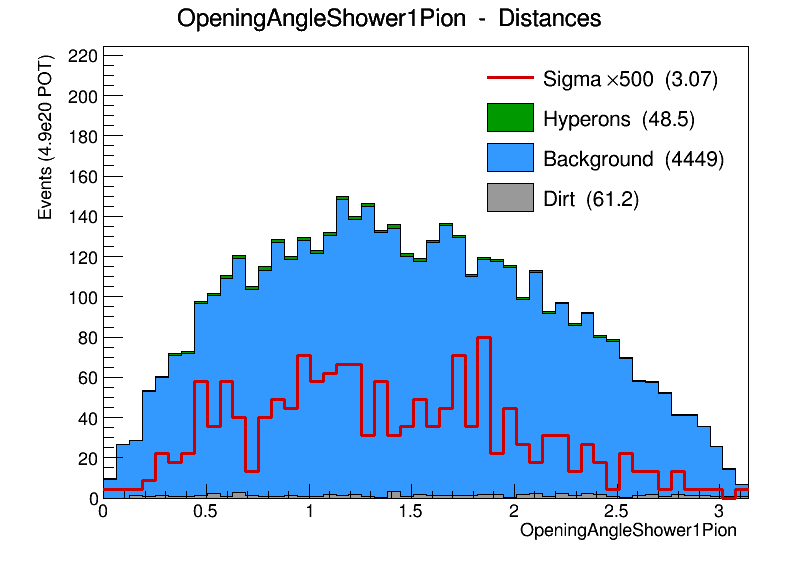
\includegraphics[width=0.31\textwidth]{../figs/stack/Distances/OpeningAngleShower1Pion.png}\hfill
  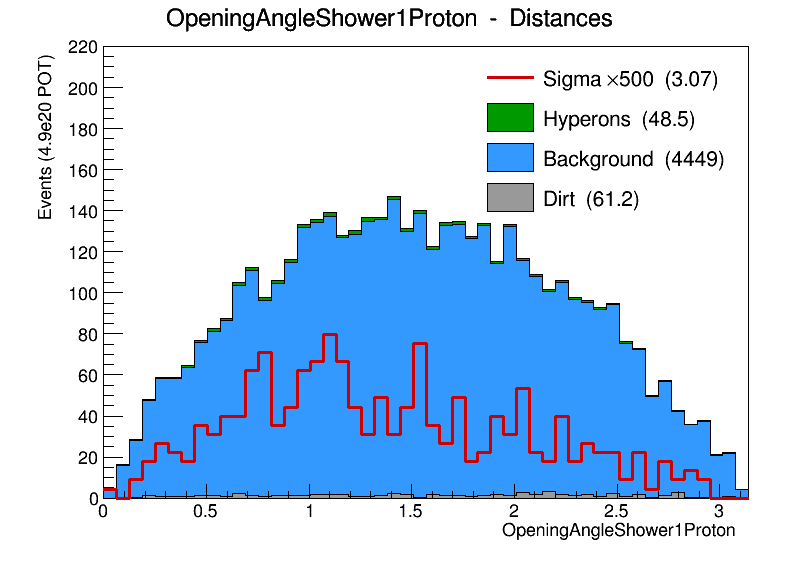
\includegraphics[width=0.31\textwidth]{../figs/stack/Distances/OpeningAngleShower1Proton.png}
  \caption{Opening angles between shower~1 and tracks:
           $\angle(\gamma_1,\mu)$ (left), $\angle(\gamma_1,\pi)$ (centre),
           $\angle(\gamma_1,p)$ (right).}
\end{figure}
\begin{figure}[H]
  \centering
  \includegraphics[width=0.31\textwidth]{../figs/stack/Distances/MuonPID.png}\hfill
  \includegraphics[width=0.31\textwidth]{../figs/stack/Distances/PionPID.png}\hfill
  \includegraphics[width=0.31\textwidth]{../figs/stack/Distances/ProtonPID.png}
  \caption{LLR PID scores at the pre-MVA stage: muon (left),
           pion (centre), proton (right).}
\end{figure}
\begin{figure}[H]
  \centering
  \includegraphics[width=0.31\textwidth]{../figs/stack/Distances/MuonTrkLength.png}\hfill
  \includegraphics[width=0.31\textwidth]{../figs/stack/Distances/PionMeanDeDxPlane2.png}\hfill
  \includegraphics[width=0.31\textwidth]{../figs/stack/Distances/ProtonMeanDeDxPlane2.png}
  \caption{Track length and calorimetry: muon track length (left),
           pion $\langle dE/dx\rangle$ collection plane (centre),
           proton $\langle dE/dx\rangle$ collection plane (right).}
\end{figure}
\begin{figure}[H]
  \centering
  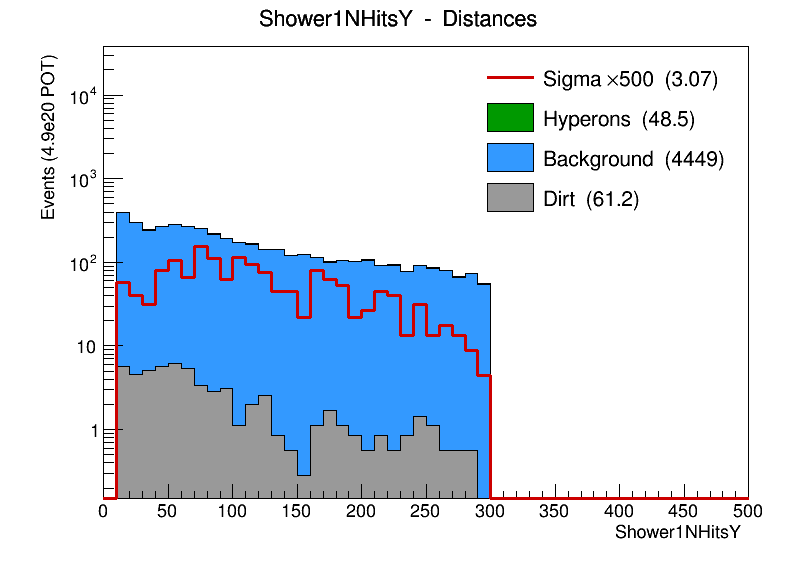
\includegraphics[width=0.31\textwidth]{../figs/stack/Distances/Shower1NHitsY.png}\hfill
  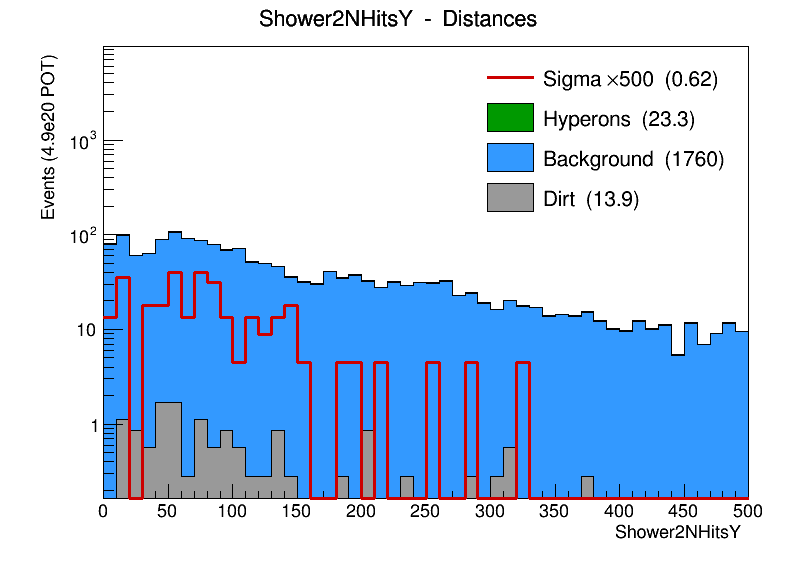
\includegraphics[width=0.31\textwidth]{../figs/stack/Distances/Shower2NHitsY.png}\hfill
  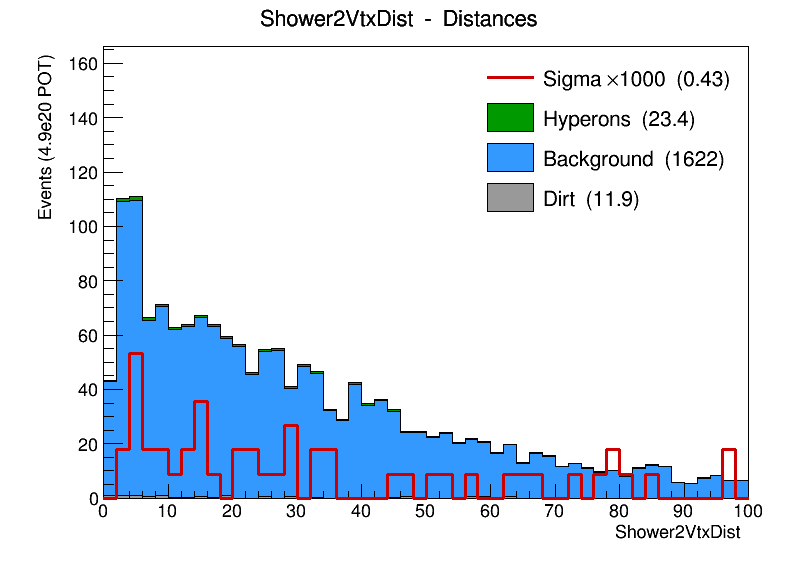
\includegraphics[width=0.31\textwidth]{../figs/stack/Distances/Shower2VtxDist.png}
  \caption{Shower variables at the pre-MVA stage: leading-shower
           collection-plane hits (left), second-shower hits (centre),
           second-shower vertex distance (right).}
\end{figure}

%% ----------------------------------------------------------
\subsection{After BDTg Selection (\texttt{BDTg}$>0.96$)}
%% ----------------------------------------------------------

\begin{figure}[H]
  \centering
  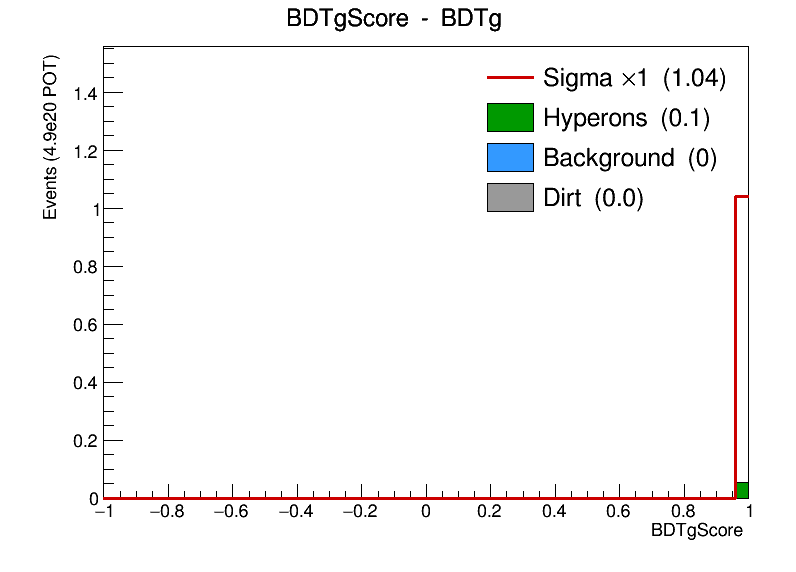
\includegraphics[width=0.31\textwidth]{../figs/stack/BDTg/BDTgScore.png}\hfill
  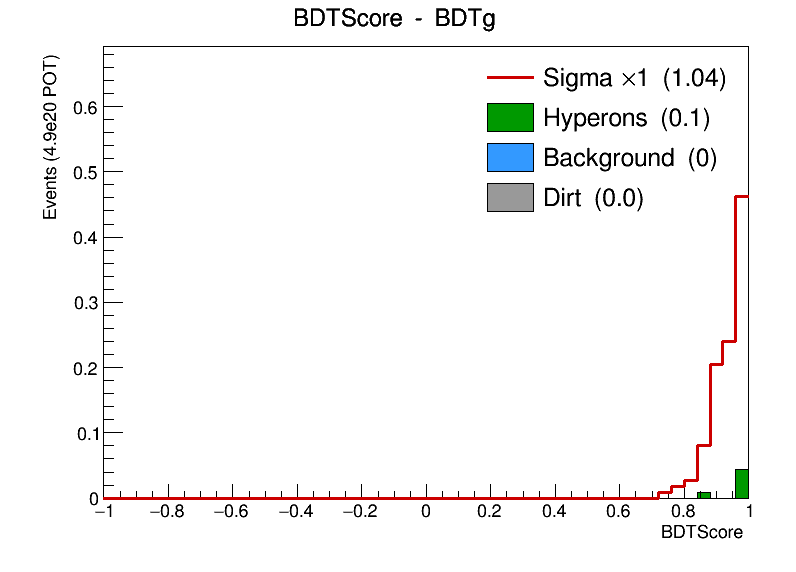
\includegraphics[width=0.31\textwidth]{../figs/stack/BDTg/BDTScore.png}\hfill
  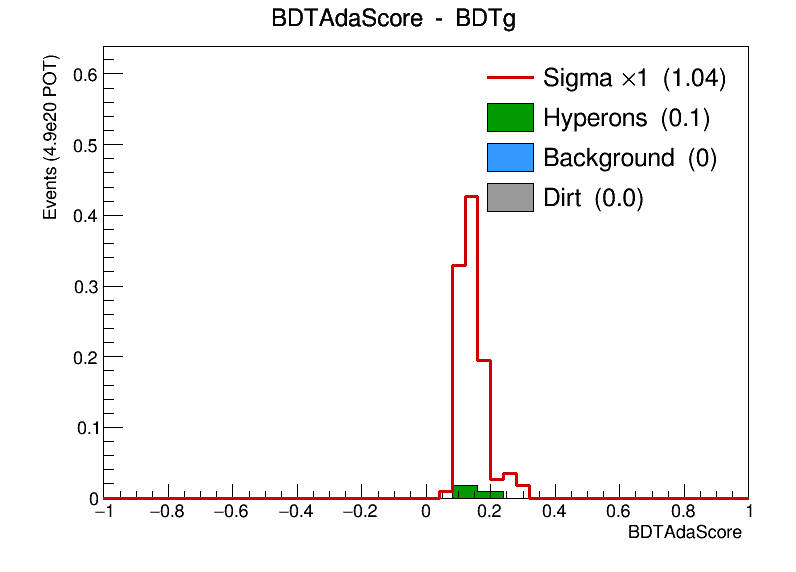
\includegraphics[width=0.31\textwidth]{../figs/stack/BDTg/BDTAdaScore.png}
  \caption{BDT classifier output scores after the final selection:
           \texttt{BDTg} (left), \texttt{BDT} (centre),
           \texttt{BDTAda} (right).  Only signal and a small residual
           hyperon contribution survive the \texttt{BDTg}$>0.96$ cut.}
\end{figure}

% ============================================================
\section{Selection Efficiency as a Function of True Momentum}
\label{app:efficiency}
% ============================================================

The selection efficiency is evaluated on the signal Monte Carlo sample as a
function of the true momentum of each final-state particle in the decay chain
$\bar{\nu}_\mu + \text{Ar} \to \mu^+ + \Sigma^0$,\;
$\Sigma^0 \to \Lambda + \gamma$,\;
$\Lambda \to p + \pi^-$.
Two cumulative selection levels are shown:
\begin{itemize}
  \item \textbf{Pre-MVA}: all pre-selection and topological distance cuts applied
        (cut level 10 in the sequence of Section~\ref{sec:selection}).
  \item \textbf{Final}: additionally requiring $\text{BDTg} > 0.96$.
\end{itemize}

The denominator in all cases is the set of true signal events satisfying the
truth-level fiducial volume requirement (Section~\ref{sec:selection}).  The
efficiency and its 68\% Bayesian (uniform prior) confidence interval are
computed with \texttt{TEfficiency}.

\begin{figure}[htbp]
  \centering
  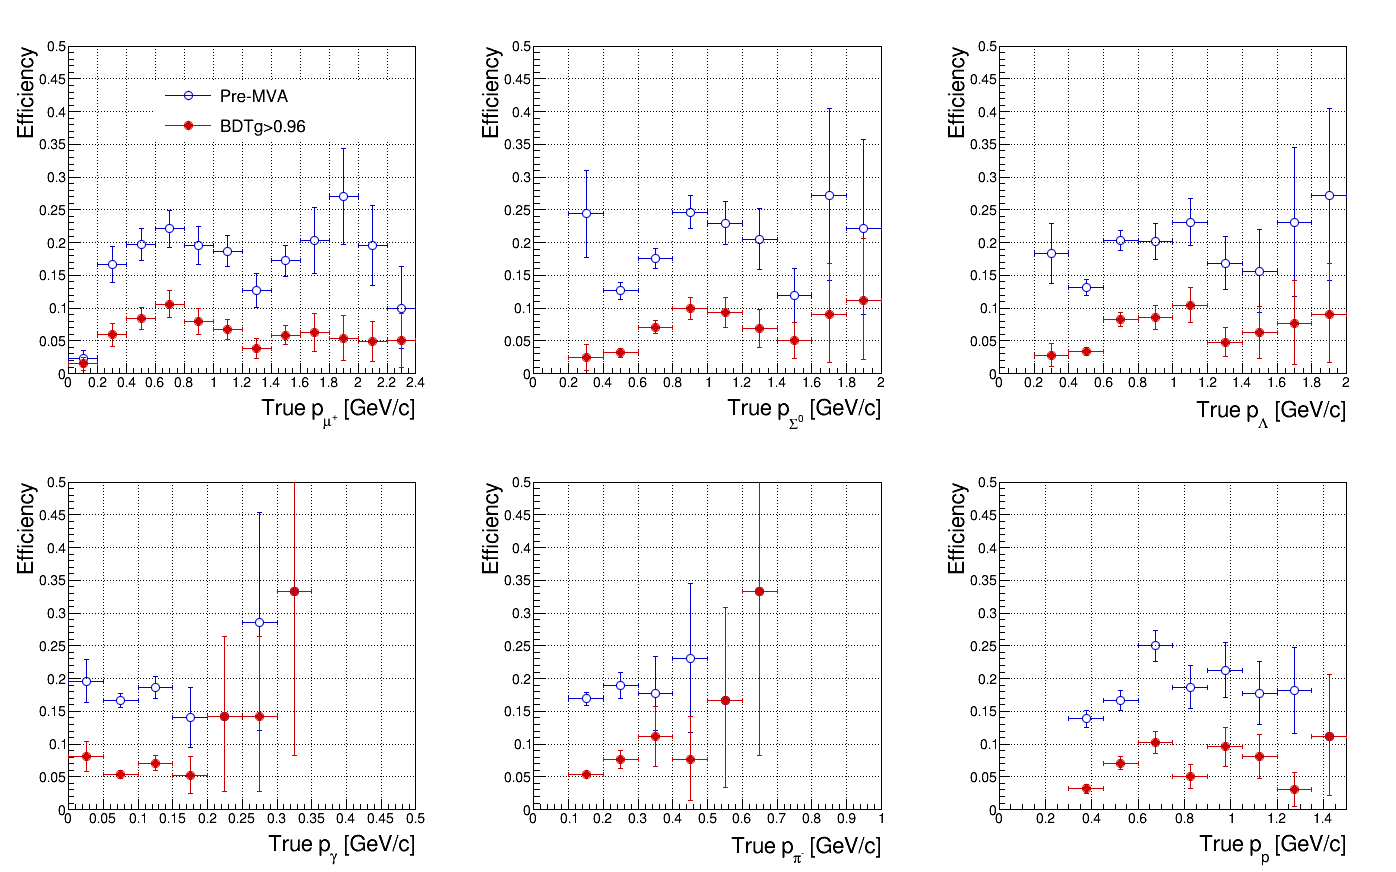
\includegraphics[width=\textwidth]{../figs/EfficiencyPlots/Eff_All.png}
  \caption{Selection efficiency as a function of true momentum for all six
           final-state particles.  Blue open circles: after all pre-selection
           and distance cuts.  Red filled circles: after the final
           $\text{BDTg}>0.96$ requirement.  Error bars indicate 68\% Bayesian
           confidence intervals.}
  \label{fig:eff_all}
\end{figure}

\subsection*{Individual particle efficiencies}

\begin{figure}[htbp]
  \centering
  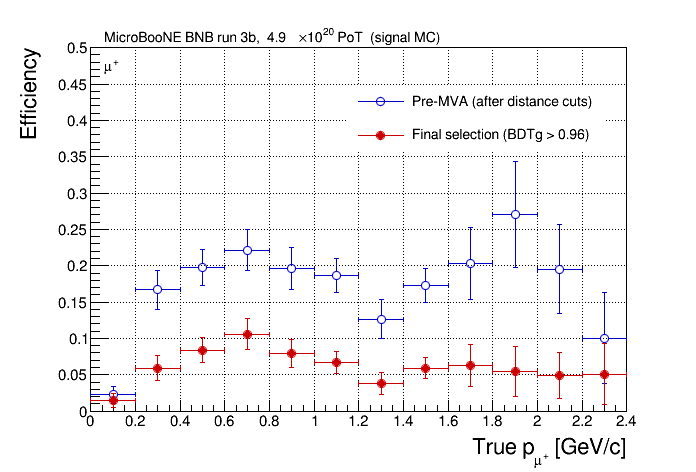
\includegraphics[width=0.48\textwidth]{../figs/EfficiencyPlots/Eff_Muon.png}
  \hfill
  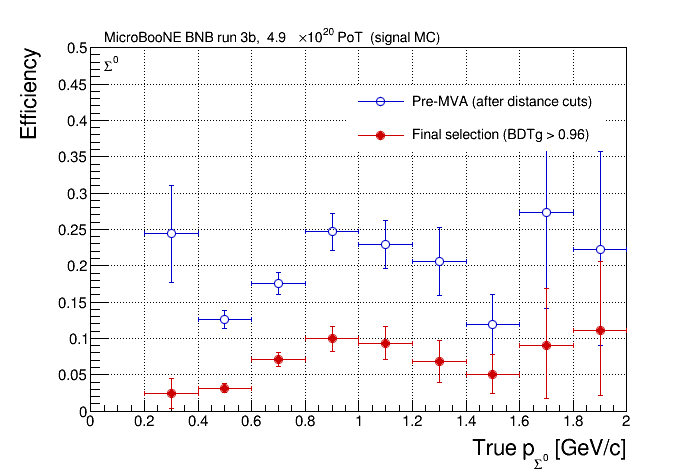
\includegraphics[width=0.48\textwidth]{../figs/EfficiencyPlots/Eff_Sigma0.png}
  \caption{Left: efficiency vs.\ true $\mu^+$ momentum.
           Right: efficiency vs.\ true $\Sigma^0$ momentum.}
  \label{fig:eff_mu_sig}
\end{figure}

\begin{figure}[htbp]
  \centering
  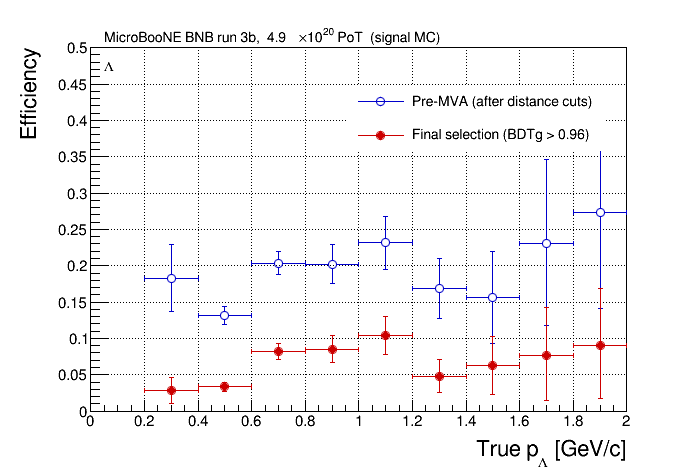
\includegraphics[width=0.48\textwidth]{../figs/EfficiencyPlots/Eff_Lambda.png}
  \hfill
  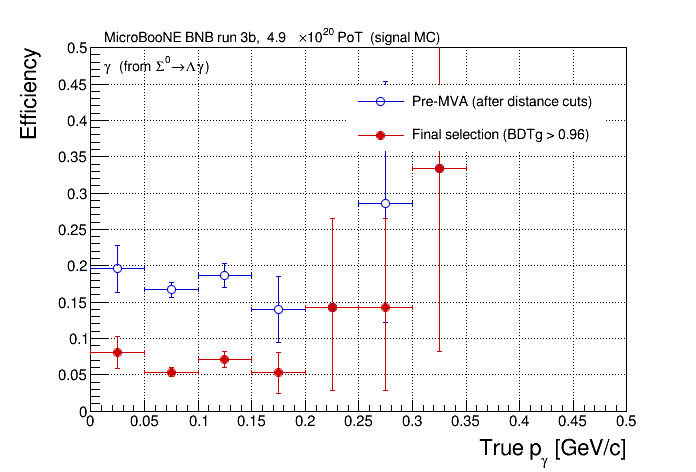
\includegraphics[width=0.48\textwidth]{../figs/EfficiencyPlots/Eff_Photon.png}
  \caption{Left: efficiency vs.\ true $\Lambda$ momentum.
           Right: efficiency vs.\ true photon momentum from
           $\Sigma^0 \to \Lambda\gamma$.}
  \label{fig:eff_lam_gam}
\end{figure}

\begin{figure}[htbp]
  \centering
  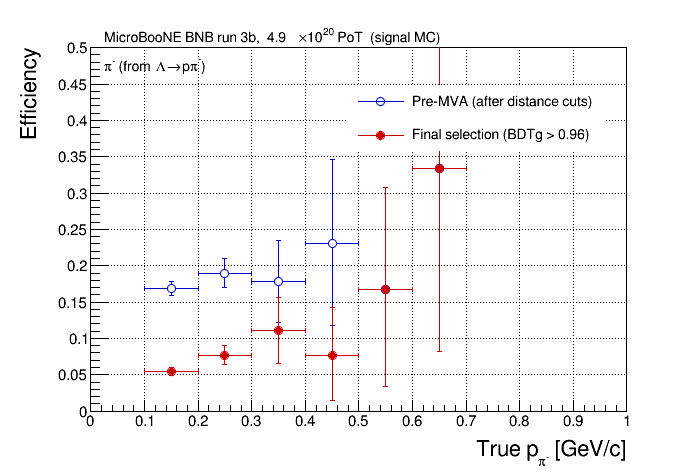
\includegraphics[width=0.48\textwidth]{../figs/EfficiencyPlots/Eff_Pion.png}
  \hfill
  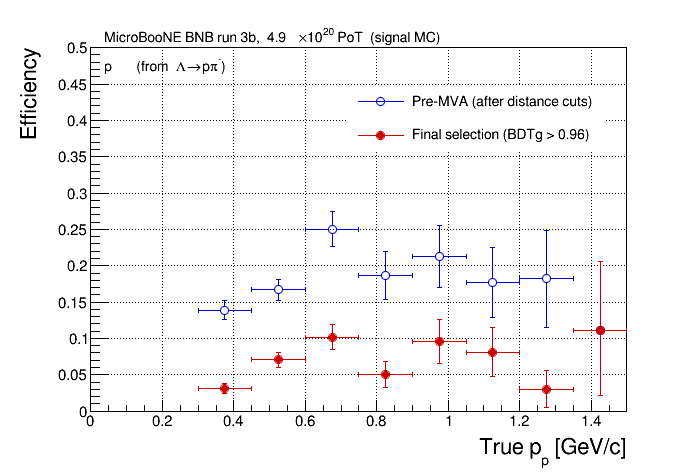
\includegraphics[width=0.48\textwidth]{../figs/EfficiencyPlots/Eff_Proton.png}
  \caption{Left: efficiency vs.\ true $\pi^-$ momentum from
           $\Lambda \to p\pi^-$.
           Right: efficiency vs.\ true proton momentum.}
  \label{fig:eff_pi_pr}
\end{figure}

The efficiency rises steeply at low momentum, reflecting the kinematic
thresholds in the signal definition ($p_p > 0.3$\,GeV/$c$,
$p_{\pi^-} > 0.1$\,GeV/$c$) and the minimum track-length requirements for
muon and pion identification.  The BDTg cut reduces the pre-MVA efficiency by
roughly a factor of two, while providing strong background suppression as
discussed in Section~\ref{sec:mva}.

\end{document}
